\documentclass[11pt, oneside, a4paper]{memoir}

%Font encoding
\usepackage[utf8]{inputenc}
\usepackage[T1]{fontenc}
\usepackage{lmodern}

%Biblio
\usepackage[backend=biber, 
			style=alphabetic, 
			isbn=false,
			doi=false,
			url=false,
			backref=false,
			giveninits=false, 
			maxcitenames=2,
			maxbibnames=100]{biblatex}
\usepackage{csquotes}

\addbibresource{./bib/manteaux.bib}
\addbibresource{./bib/arps-vriphys2013.bib}
\addbibresource{./bib/cutting-mig2015.bib}

\usepackage[colorlinks=true,
            linkcolor=blue,
            urlcolor=blue,
            citecolor=blue]{hyperref}

%Maths
\usepackage{amsmath}

%Images
\ifpdf \usepackage[pdftex]{graphicx} \pdfcompresslevel=9
\else \usepackage[dvips]{graphicx} \fi

%Color and highlighting
\usepackage{transparent}
\usepackage{soul} % highlighting with word wrap
\newcommand{\highlight}[2]{\colorlet{hlcolor}{#1}\sethlcolor{hlcolor}\hl{#2}} % work around soul/xcolor conflict
\usepackage[usenames,dvipsnames]{xcolor}

%Math commands
\renewcommand{\vec}[1]{\mathbf{#1}}
\newcommand{\vp}{\vec p}
\newcommand{\vq}{\vec q}
\renewcommand{\H}{\mathcal{H}}

%Algorithms
\usepackage{algorithm}
\usepackage{algpseudocode}
\algnewcommand{\LineComment}[1]{\State \(\triangleright\) #1}

%Improvement
\usepackage[activate={true,nocompatibility},
			final,tracking=true,
			kerning=true,
			spacing=true,
			factor=1000,
			stretch=10,
			shrink=10]{microtype}
\microtypecontext{spacing=nonfrench}

%Subfigure
\usepackage{subcaption}

%Highlighting command
\newcommand{\TODO}[1]{\highlight{Orange!40}{TODO: #1}}

%Table of contents settings
\settocdepth{subsubsection}
\setsecnumdepth{subsection}

%Titles
%\usepackage{titlesec}	

%Table of contents
%\usepackage{titletoc}

% activate={true,nocompatibility} - activate protrusion and expansion
% final - enable microtype; use "draft" to disable
% tracking=true, kerning=true, spacing=true - activate these techniques
% factor=1100 - add 10% to the protrusion amount (default is 1000)
% stretch=10, shrink=10 - reduce stretchability/shrinkability (default is 20/20)

\begin{document}

\title{Simulation and control of physical phenomena}
\author{Pierre-Luc Manteaux}
\date{\today}
\maketitle

\frontmatter

%\chapter{Remerciements}
%Merci

\chapter{R\'esum\'e}
Dans ce document nous pr\'esentons des techniques pour la simulation efficace et le contr\^ole de ph\'enom\`enes physiques.

\chapter{Abstract}
In this document we present techniques for the efficient simulation and control of physical phenomena.

\tableofcontents

\mainmatter

\chapter{Introduction}
An introduction.

\section{Problems}
\begin{itemize}
    \item Non-intrusive adaptive techniques for physics-based animation.
    \item Plausible and efficient simulation of detailed topological changes with very few degrees of freedom.
    \item Study of adaptive models for physics-based animation.
    \item Modeling of animations from existing animations.
\end{itemize}

\section{Contributions}
\begin{itemize}
    \item Transfer of adaptive techniques from Nanosystems simulation to Computer Graphics.
    \item Algorithm for the efficient cutting of thin deformable objects using the frame-based model.
    \item Algorithm for the modeling of fluid animation.
\end{itemize}

\section{Collaborations}

\begin{itemize}
    \item Wei-Lun Sun
    \item Julio Toss
    \item Thibault Lejemble, Amélie Fondevilla, Thibault Blanc-Beyne, Nicolas Durin
    \item Ulysse Vimont
\end{itemize}

\section{Structure of the document}
Overview of the manuscript

\section{Related publications}
Some publications.
\begin{itemize}
    \item \cite{Manteaux2013}
    \item \cite{Lejemble2015}
    \item \cite{Manteaux2015}
\end{itemize}

\chapter{Notation}

\begin{table}[!h]
\begin{tabular}{ll}
$t$ & time \\
$m$ &  mass \\
$\mathbf{x}$ & position \\
$\mathbf{v}$ & velocity \\
$\mathbf{f}$ & total forces \\
$\mathbf{f}_{int}$ & internal forces \\
$\mathbf{f}_{ext}$ & external forces \\
\end{tabular}
\end{table}

\chapter{State of the art}
A nice state of the art.

\section{Continuum mechanics}
\subsection{Equations of motion}
\subsubsection{Conservation of mass}
\subsubsection{Conservation of momentum}
\subsubsection{Constitutive Law}
\subsubsection{Spatial discretization}
\paragraph{Interpolation}
\paragraph{Integration}
\subsubsection{Temporal integration}
\paragraph{Explicit}
\paragraph{Implicit}
\subsection{Solid mechanics}
\subsubsection{Constitutive Law}
\subsubsection{Frame-based model}
\subsection{Fluid mechanics}
\subsubsection{Constitutive Law}
\subsubsection{SPH model}
\section[A quick \& dirty introduction to fluid dynamics]{A quick \& dirty introduction to computational fluid dynamics}

\subsection{Navier-Stokes equation}

\paragraph{Mass conservation}
The conservation of mass is quite explicit. The mass of the fluid cannot change. Mathematically, it is expressed by stating that the variation of the mass in a given volume is equal to the flux of mass going through the border of the volume.
\begin{equation}
    \label{eq:massConservation}
    \frac{d}{dt}\left( \int_{\mathcal{V}} \rho dx \right)
    =
    - \int_{\mathcal{\partial V}}\rho \mathbf{v} \mathbf{n} ds
\end{equation}

From Stokes' formula, we have

\begin{equation}
\int_{\partial \mathcal{V}} \rho \mathbf{v} \mathbf{n} ds =
\int_{\mathcal{V}} \nabla \cdot \left( \rho \mathbf{v} \right)
\end{equation}

then the conservation of mass can be rewritten as

\begin{equation}
\int_{\mathcal{V}} \frac{d}{dt} \rho + \nabla \cdot \left( \rho  \mathbf{v} \right) dx = 0
\end{equation}

\paragraph{Constitutive Law}
The constitutive law describes how the fluid react to a deformation. For an incompressible fluid, the fluid reacts to pressure and viscosity and can be written:
\begin{equation}
\sigma = -pI + \eta \left( \nabla \mathbf{v} + \nabla \mathbf{v}^{T} \right)
\end{equation}

\paragraph{Incompressibility}
This states that the mass should not vary over time. Then the mass conservation can be rewritten as:
\begin{equation}
\nabla \cdot u = 0
\end{equation}

\paragraph{Momentum conservation}

Also called Newton's second law, it states:
\begin{equation}
\label{eq:momentumConservation}
\int_{\mathcal{V}} \rho \frac{D}{Dt} \mathbf{v}(t,x) dx = \int_{V} \mathbf{f} dx
\end{equation}

Two kind of forces are generally applied on a fluid, the \emph{external} forces and the \emph{internal} forces.

External forces describe the action of the surrounding environment on the fluid, the simplest example is the gravity:
\begin{equation}
\int_{\mathcal{V}} \rho \mathbf{g} dx
\end{equation}

Internal forces describe the reaction of the fluid to an external deformation. A general way to describe them is by using a tensor notation:
\begin{equation}
\int_{\mathcal{V}} \sigma \mathbf{n} ds
\end{equation}
By applying the Stokes' formula we can describe it with respect to the volume:
\begin{equation}
\int_{\mathcal{V}} \sigma \mathbf{n} ds =
\int_{\mathcal{V}} \nabla \cdot \sigma dx
\end{equation}

Conservation of momentum can then be rewritten:
\begin{equation}
\int_{\mathcal{V}} \rho \frac{D}{Dt} \mathbf{v}(t,x) dx = \int_{V} \rho \mathbf{g} + \nabla. \sigma dx
\end{equation}

Then we have:
\begin{equation}
\nabla \cdot \sigma = \nabla \cdot \left( -pI + \eta \left( \nabla \mathbf{v} + \nabla \mathbf{v}^{T} \right) \right) = -\nabla p + \Delta \mathbf{v}
\end{equation}

With internal forces, we have the Navier-Stokes equation for an incompressible fluid:

\begin{equation}
\begin{array}{ll}
\int_{\mathcal{V}} \rho \frac{D}{Dt} \mathbf{v}(t,x) dx = \int_{V} \rho \mathbf{g} -\nabla p + \eta \Delta \mathbf{v} dx \\
\nabla. \mathbf{u} = 0
\end{array}
\end{equation}

\paragraph{Lagrangian vs Eulerian}

Lagrangian: You follow the river. The river is discretized into particles which carries and update fluid properties such as position and velocity. 

Eulerian : You stand in the middle of a river. The river is discretized into a fixed grid from where you can measure the velocity of the flow passing through the point of the grid.

The material derivative:
\begin{equation}
\frac{D\mathbf{u}}{Dt} = \frac{\partial \mathbf{u}}{\partial t} + (\mathbf{u} \cdot \nabla v)
\end{equation}

In a lagrangian framework, the positions of the particles at a specific time $t$ is known, so the material derivative is just the time derivative.

\begin{equation}
\frac{D\mathbf{u}}{Dt} = \frac{\partial u}{\partial t}
\end{equation}

Moreover, if we assume that the mass of the particles is constant through the simulation, then conservation of mass is granted and we can omit its numerical solving. However, in practice it does not ensure that the divergence of the velocity will be null, new methods were proposed to enforce the null divergence condition. In this work we keep the first approximation and do not enforce the null divergence condition.

\subsection{Discretization}

Once equations of motion have been set, they can be discretized in space and time and integrated.

\subsection{Discretization: The Smoothed Hydrodynamics Particles model}
Smoothed Particles Hydrodynamics is an interpolation method that can be used to discretize the Navier-Stokes equation in a Lagrangian way. The fluid is discretized into particles which represent a small volume of the whole fluid and each quantity is interpolated using SPH.

\paragraph{SPH interpolation}
The interpolation of a function $f$ at a position $\mathbf{x}$ is :
\begin{equation}
f(\mathbf{x}) = \int_{V} f(\mathbf{x'})W(\mathbf{x}-\mathbf{x'}, h)dx'
\end{equation}
where $W$ is a function called \emph{kernel}. 

If the fluid is discretized into particles with a mass $m$, a density $\rho$ and a volume $V$, then we can discretize the SPH interpolation as:
\begin{equation}
f(\mathbf{x}) = \sum_{p} f(\mathbf{x}_{p})V_{p} W(\mathbf{x}-\mathbf{x_{p}},h) = \sum_{p} f(\mathbf{x}_{p})\frac{m_{p}}{\rho_{p}} W(\mathbf{x}-\mathbf{x_{p}},h)
\end{equation}

Then derivatives can be computed and discretized the same way:
\begin{equation}
D^{\alpha} f(\mathbf{x}) = \int_{\mathcal{V}} f(\mathbf{x'}) D^{\alpha} W(\mathbf{x}-\mathbf{x'}, h)dx'
\end{equation}

\begin{equation}
D^{\alpha} f(\mathbf{x})= \sum_{p} f(\mathbf{x}_{p})\frac{m_{p}}{\rho_{p}} D^{\alpha} W(\mathbf{x}-\mathbf{x_{p}},h)
\end{equation}

However, for first derivatives, the approximation does not vanish if $f$ is constant. A quick way to ensure that is to use a differentiable function $\Phi$ (in practice we use the density $\rho$) to re-write the derivative using the derivative of a product :
\begin{equation}
\nabla f(x) = \frac{1}{\Phi}\left(\nabla (f \Phi) - f \nabla \Phi \right)
\end{equation}

\paragraph{How to choose the kernel}
The properties of $W$ can vary with respect to the properties of the function to be interpolated. In general, $W$ meet the following properties:
\begin{itemize}
\item $W$ is normalized. Thus, constants are interpolated exactly.
\item $W$ has a compact support.
\begin{equation}
\parallel \mathbf{x} \parallel \geq h \rightarrow W(\mathbf{x},h) = 0 
\end{equation}
\begin{equation}
\int_{\mathcal{V}} W(\mathbf{x},h) dx = 1
\end{equation}
\item $W$ tend to the delta function when the length scale $h$ tends to $0$.
\begin{equation}
\lim_{h \rightarrow 0} W(x,h) = \delta(x)
\end{equation}
\item $W$ should be symmetric to enforce invariance under rotation
\begin{equation}
W(-x,h) = W(x,h)
\end{equation}
\item Depending on the function to interpolate the kernel should be positive to prevent unphysical interpolated value.
\begin{equation}
W \geq 0
\end{equation}
\end{itemize}

The cubic kernel from Monaghan is a good choice in practice.

\paragraph{Applications to Navier-Stokes}

\begin{equation}
\rho_{i} = \sum_{j} m_{j}W(\mathbf{x_{j}}-\mathbf{x_{j}},h)
\end{equation}

\begin{equation}
\left(\nabla p\right)_{i} = \sum_{j} \frac{m_{j}}{\rho_{j}} p_{j} \nabla W(\mathbf{x_{j}}-\mathbf{x_{j}},h)
\end{equation}

However linear and angular momentum are not conserved as the formula is not symmetric. By using the previous technique with $\Phi = \frac{1}{\rho}$, it can be symmetrized:

\begin{equation}
\left(\nabla p\right)_{i} = 
\frac{1}{\rho_{i}}
\sum_{j} m_{j} \left( \frac{p_{i}}{\rho_{i}^{2}} + \frac{p_{j}}{\rho_{j}^{2}} \right) \nabla W(\mathbf{x_{j}}-\mathbf{x_{j}},h)
\end{equation}

\begin{equation}
\left(\Delta \mathbf{v}\right)_{i} = \sum_{j} \frac{m_{j}}{\rho_{j}} \mathbf{v}_{j} \Delta W(\mathbf{x_{j}}-\mathbf{x_{j}},h)
\end{equation}

Same as for the pressure gradient, this is not symmetric. Here it can be symmetrized by using $\Phi = \rho$.

\begin{equation}
\left(\Delta \mathbf{v}\right)_{i} = \frac{1}{\rho_{i}}\sum_{j} m_{j} \left( \mathbf{v}_{j}-\mathbf{v}_{i}\right) \Delta W(\mathbf{x_{j}}-\mathbf{x_{j}},h)
\end{equation}

In practice, the evaluation of the laplacian is not accurate. Another form of viscosity based on the gradient was proposed. This is still an area of research.

\begin{equation}
\left(\Delta v\right)_{i} = 
\frac{1}{\rho_{i}}
\sum_{j} m_{j} \Pi_{ij} \nabla W(\mathbf{x_{j}}-\mathbf{x_{j}},h)
\end{equation}

where 

\begin{equation}
\Pi_{ij} = -\frac{2hc_{s}}{\rho_{i}+\rho_{j}}\frac{v_{ij}^{T}x_{ij}}{\vert x_{ij} \vert^{2} + \epsilon h^{2}}
\end{equation}

Now if we discretize Navier-Stokes for one particle $i$, we have:

\begin{equation}
m_{i}\frac{d}{dt}v_{i}(t) = m_{i}\mathbf{g} - m_{i}(\nabla p)_{i} + m_{i}(\delta \mathbf{v})_{i}
\end{equation}

This equation can now be discretized in time and integrated. In practice we use the euler symplectic integrator:

\begin{equation}
\begin{array}{ll}
v_{i}(t+\Delta t) = v_{i}(t) + \Delta t \frac{d}{dt}v_{i}(t) \\
x_{i}(t+\Delta t) = x_{i}(t) + \Delta t v_{i}(t+\Delta t)
\end{array}
\end{equation}

Several interesting implementation problems arise when dealing with particle system and more particularly particle-based fluid simulations:

\begin{itemize}
\item Boundary handling 
\item Surface reconstruction
\item Optimization (acceleration structure for spatial query)
\end{itemize}

Faire un tableau avec les références et ce que l'on peut y trouver d'intéressant.

%\paragraph{Eulerian grid}
%\paragraph{Lagrangian particles}
%\paragraph{Hybrid method}
%\paragraph{Smoothed Hydrodynamics Particles model}

\section[A quick \& dirty introduction to continuum mechanics]{A quick \& dirty introduction to continuum mechanics}

The behavior of an elastic deformable model is described by conservation laws and a constitutive law.

The first conservation law is the conservation of mass.

The second conservation law is the conservation of momentum.

The constitutive law depict the behavior of the object with respect to a deformation.

\begin{equation}
\begin{array}{ll}
\int_{\mathcal{V}} \frac{d\mathbf{v}}{dt} = \int_{\mathcal{V}} \rho \mathbf{g} + \nabla \cdot \sigma dx 
\\
\int_{\mathcal{V}} \nabla \cdot u = 0
\end{array}
\end{equation} 

A common way to describe the stress tensor for elastic materials is to use a constitutive density energy:
\begin{equation}
\sigma = \frac{\partial \Psi}{\partial \epsilon}
\end{equation}

There are many forms of enery. For a classical Hookean material, the density energy is
\begin{equation}
\Psi = \frac{1}{2}H\epsilon^{2}
\end{equation}

Then the stress tensor is
\begin{equation}
\sigma = H\epsilon
\end{equation}

H is called the stiffness tensor and is a $3\times3\times3\times3$ tensor. For isotropic materials, the number of material parameters can be reduced to two, the Young's modulus $E$ and the Poisson's ratio $\nu$. Also, the strain and stress tensor being symmetric, the constitutive law can be simplified:
\begin{equation}
\sigma = 
\begin{bmatrix}
\sigma_{11} \\
\sigma_{22} \\
\sigma_{33} \\
\sigma_{23} \\
\sigma_{13} \\
\sigma_{12}
\end{bmatrix}
=
\tilde{H}
\begin{bmatrix}
\epsilon_{11} \\
\epsilon_{22} \\
\epsilon_{33} \\
2\epsilon_{23} \\
2\epsilon_{13} \\
2\epsilon_{12}
\end{bmatrix}
\end{equation}

where

\begin{equation}
\tilde{H} =
\frac{E}{\left(1+\nu\right)\left(1-2\nu\right)}
\begin{bmatrix}
1-\nu & \nu & \nu & 0 & 0 & 0 \\ 
\nu & 1-\nu & \nu & 0 & 0 & 0 \\
\nu & \nu & 1-\nu & 0 & 0 & 0 \\
0 & 0 & 0 & \frac{1-2\nu}{2} & 0 & 0 \\
0 & 0 & 0 & 0 & \frac{1-2\nu}{2} & 0 \\
0 & 0 & 0 & 0 & 0 & \frac{1-2\nu}{2} \\
\end{bmatrix}
\end{equation}

The strain is used to measure the relative deformation with respect to the rest position of the object: elongation, compression. Therefore it is  linked to the variation of position of the object. In 3D, this position is described by 3 coordinates which can be derived with respect to each direction, then the strain should be represented by a $3\times3$ matrix.

An object is deformed if it has been compressed, stretched or sheared. The strain should measure this deformation and be $0$ when the object is at its rest position. This constraint can be expressed as:
\begin{equation}
\epsilon = \left( \nabla \mathbf{x} \right)^{T} \nabla \mathbf{x} - I
\end{equation}

$\nabla \mathbf{x}$ is also called deformation gradient.

For elastic object, the position is always relative to the rest position. Therefore, a displacement vector is often used to depict the current position.
\begin{equation}
\mathbf{x} = \mathbf{x}_{0} + \mathbf{u}
\end{equation}

Then the strain relation becomes
\begin{equation}
\epsilon = \nabla \mathbf{u} + \left( \nabla \mathbf{u} \right)^{T} + \left(\nabla \mathbf{u}\right)^{T}\nabla \mathbf{u}
\end{equation}

It is called the Green-Lagrange strain and its linearized version the Cauchy strain.

\begin{equation}
\epsilon = \nabla \mathbf{u} + \left( \nabla \mathbf{u} \right)^{T}
\end{equation}

The strain measurement is the big difference with respect to fluid dynamics because it is the link between the deformed object and its rest shape whereas there are no such thing when computing the stress for a fluid.

Now we are ready to discretize the equations of motion in space and time.

\paragraph{Discretization}

Now that we have a clear description of the equation of motions, we can discretize them in space and time. Here a large number of methods can be used. 

Spatial discretization are divided into two categories: mesh-based and meshfree. For both of them, different kind of degrees of freedom can be chosen. For both of them, different interpolation methods can be chosen. 

Here we focus on a method called the frame-based model. The degrees of freedom are affine frames and the interpolation method is based on a method called linear blend skinning.

Affine frames represent $9$ degree of freedoms, $3$ for translation, $3$ for rotation and $3$ for scaling. They uniformly sample the object and are used to compute the dynamics.

For elastic objects, we need to build a mapping between the rest shape $\Omega_{0}$ and the deformed shape of the object $\Omega$ in order to compute the deformation gradient, this is called the displacement field $\Phi$.

\begin{equation}
\begin{array}{llll}
f & \Omega_{0} & \longrightarrow & \Omega \\
	 & \mathbf{x_{0}} & \longrightarrow & \mathbf{x}
\end{array}
\end{equation}

In order to approximate this mapping, we use a set of functions called the shape functions $\left\lbrace \Phi \right\rbrace_{i}$. This set of functions should be consistent, i.e form a partition of unity :
\begin{equation}
f(\mathbf{x}) = \sum_{i} \Phi_{i}(\mathbf{x}) f(\mathbf{x}_{i})
\end{equation}

For derivatives, computation becomes straightforward:
\begin{equation}
D^{\alpha}f(\mathbf{x}) = \sum_{i} D^{\alpha}\Phi_{i}(\mathbf{x}) f(\mathbf{x}_{i})
\end{equation}

\begin{itemize}
\item Collision detection and response
\item Strain rate (viscosity)
\end{itemize}

\section{Adaptive techniques and model for physics-based animation}

\section{Control of physics-based animation}

\section{Modeling of animated physical phenomena}


\chapter{ARPS}

\begin{figure}[!h]
    \begin{tabular}{cc}
        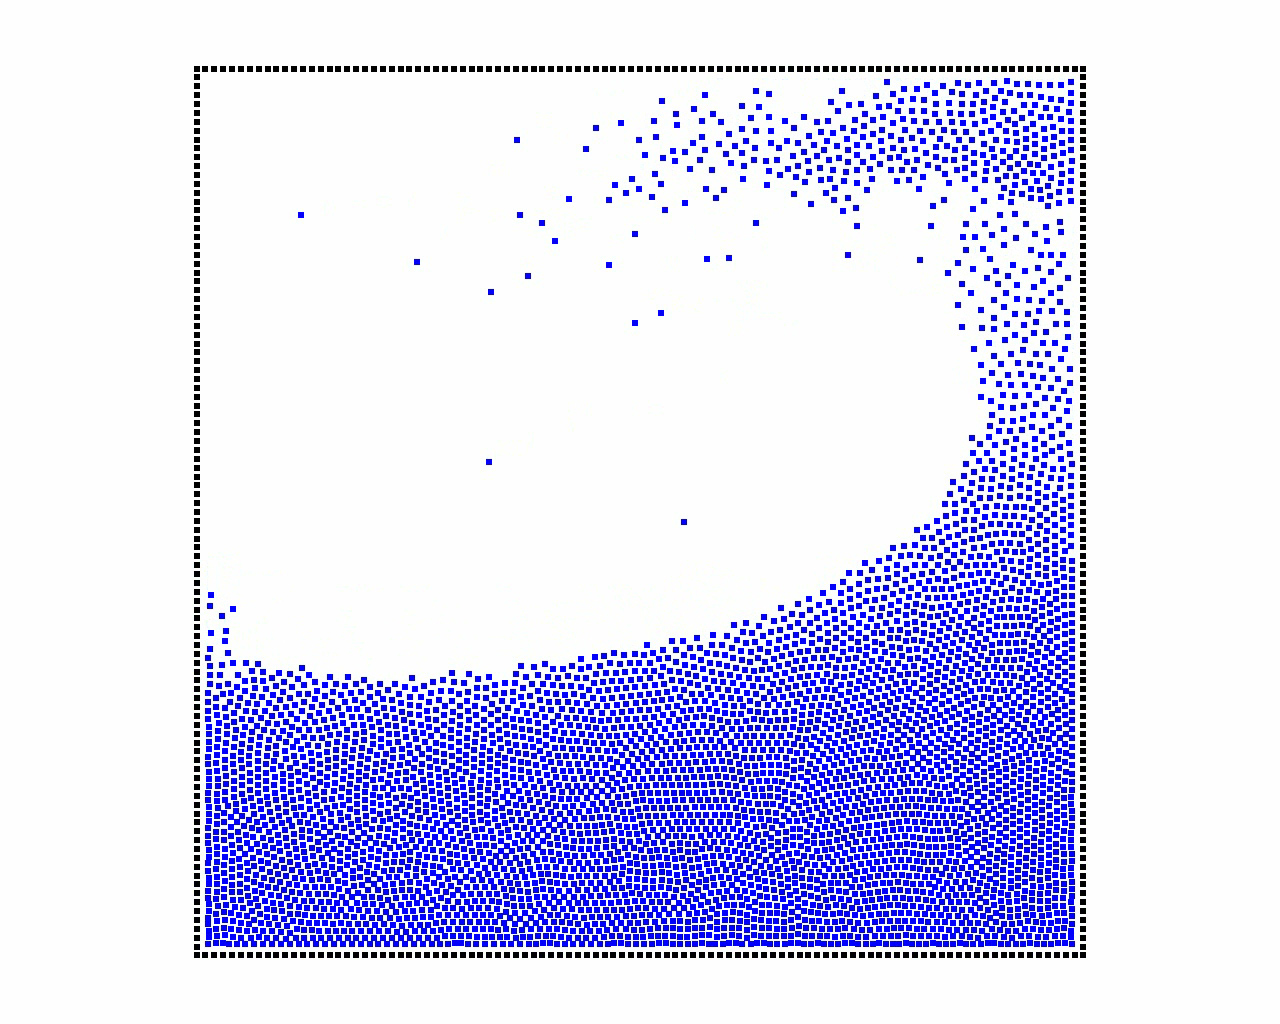
\includegraphics[width=0.4\linewidth]{images/arps-vriphys2013/ReposSPHClassique1.jpg} &
        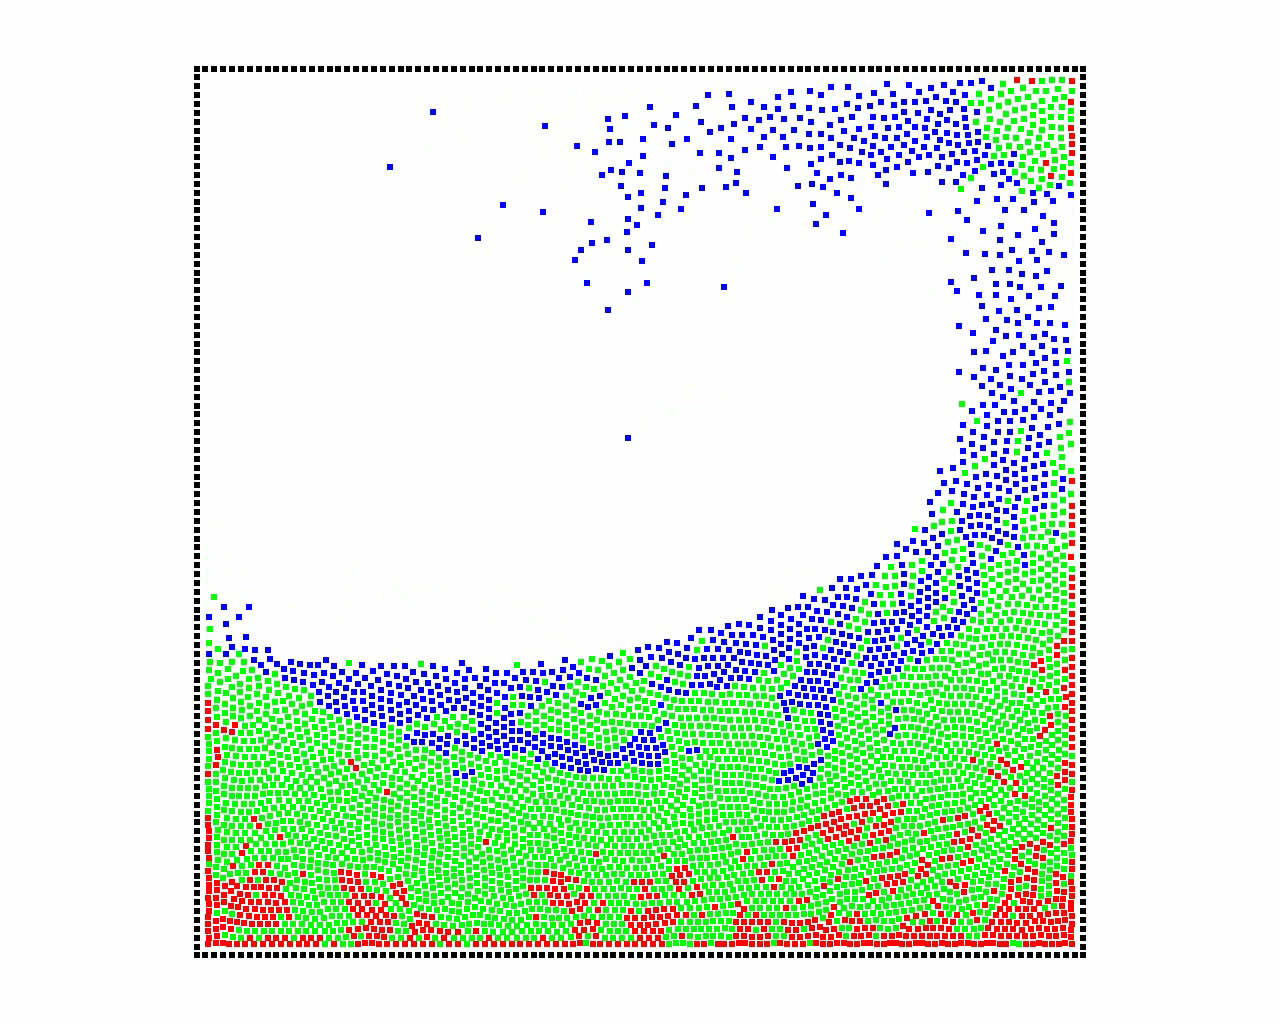
\includegraphics[width=0.4\linewidth]{images/arps-vriphys2013/ReposSPHARPSColor1.jpg}
    \end{tabular}
 \centering
 \caption{ A dam break simulation with 5000 particles simulated with WCSPH (on the left)
 and with our adaptive method (on the right). On the right image, blue corresponds to full-dynamics particles, green to transition particles and red to restrained particles.}
\label{fig:teaser}
\end{figure}

In this paper, we explore the use of Adaptively Restrained (AR) particles for graphics simulations. Contrary to previous methods,
Adaptively Restrained Particle Simulations (ARPS) do not adapt time or space sampling, but rather switch the positional degrees of freedom of particles on and off, while letting their momenta evolve. Therefore, inter-particles forces do not have to be updated at each time step, in contrast with traditional methods that spend a lot of time there.

We present the initial formulation of ARPS that was introduced for molecular dynamics simulations, and explore its potential for Computer Graphics applications:
We first adapt ARPS to particle-based fluid simulations and propose an efficient incremental algorithm to update forces and scalar fields.
We then introduce a new implicit integration scheme enabling to use ARPS for cloth simulation as well.
Our experiments show that this new, simple strategy for adaptive simulations can provide significant speedups more easily than traditional adaptive models.

%-------------------------------------------------------------------------
\section{Introduction}
Combining efficiency with visual realism had been one of the main goals of Computer Graphics research in the last decade. The general strategy for efficient graphical simulations is to concentrate the computational time on the most interesting parts of an animated scene (such as near the surface of a fluid), while simplifying the rest of the scene according to some visual quality criteria. A number of adaptive simulation methods, aimed at controlling the trade-off between performance and precision, have been developed. Most of them consist in changing time or space sampling, using adaptive time steps or multi-scale models.
Although several of them give impressive results, they are often difficult to implement, may-be restricted to specific applications, sometimes generate discontinuity artifacts due to sudden simplifications.

A different approach for adaptive simulation~\cite{Artemova2012} was recently proposed in the context of molecular dynamics~(MD).
The key idea is that since most of the computation time is spent in computing interaction forces based on positions, particles with low velocity could be considered fixed in space - and the corresponding interaction forces constant - until they accumulate enough momentum to start moving again.
While freezing objects to gain computation time has been extensively used in video games, the question of when and how to release them has not been extensively studied, and has mainly relied on \textit{ad hoc} heuristics.
Adaptively Restrained Particle Simulations~(ARPS), in contrast, introduces a physically sound approach with proven correctness, and has been successfully used in the context of predictive, energy- and momentum-conserving particle simulation.

We present the first applications of ARPS to physically-based animation, and we complement the approach with two novel extensions, to cope with the specificity of our domain.
Damping forces, not present in the classical MD framework, create specific difficulties that we tackle using a novel freeze criterion.
Additionally, we derive an implicit integration method for applying ARPS to stiff objects.
The remainder of this paper is organized as follows.
We first briefly review the previous work on adaptive mechanical simulations in computer graphics.
We then summarize the ARPS method in Section~\ref{sec arps}.
The question of damping is studied in Section~\ref{sec sph} through viscosity forces in SPH simulations.
An extension to implicit integration is presented in Section~\ref{sec cloth} using a cloth-like use case.
Practical implementation and parameter tuning are then addressed in Section~\ref{sec implementation}. We finally discuss results and perspectives in Section~\ref{sec discussion}.


% Molecular dynamics are limited by inter-particles forces computation which cost a lot of time at each time step.
% In this paper, we explore a new kind of adaptivity introduced in molecular dynamics by \cite{Artemova2012} and called \emph{Adaptively Restrained Particle Simulation (ARPS)}.
% By switching on and off positional degrees of freedom, ARPS proposes a solution to adaptively reduce the number of inter-particles forces to compute.
% \newline \newline
% We think ARPS idea can be a more general form of adaptivity and extended to deformable model.
% We study ARPS for computer graphics and identifies the main differences between molecular dynamics and computer graphics.
% We propose solutions to extend ARPS to common particle-based fluid simulations and to stiff objects.
% Implementation issues are discussed, an efficient incremental algorithm is proposed for fluid simulation and a hybrid
% integration scheme is proposed for stiff objects simulation.
%\IDEA{Une nouvelle approche dadaptativite en molecular dynamics : ARPS
%   qui a des speed up interessant.
%   \newline Un type dadaptativite peu vu en computer graphics.
%   \newline
%   Resultat interessant. Simulation de particules est loin detre etranger au computer graphics.
%   \newline Une implementation relativement simple (pas de structure compliques, \dots)
%   \newline Une idee dadaptativite exploitable au dela des particules : FEM.
%   \newline
%   Des perspectives interessantes dans des scenes complexes ou une interaction
%   locale intervient : simulation chirurgical, environnement, ...
%
%TODO{ Existing Adaptive Methods  : \begin{enumerate}
%       \item Coarse-grainin methods
%       \item Multi Resolution methods
%end{enumerate}}
%TODO{ What difference with ARPS : \begin{enumerate}
%   \item Spatial Resolution stay fixed but physics resolution
%       may be reduced. So for instance rendering technics need no
%       change, they only can benefit from the method.
%   \item Adaptivity is baked in physics not in the deformation model.
%end{enumerate} }
%-------------------------------------------------------------------------
\section{Previous work}
There have been two main ways to address adaptivity in Computer Graphics: time adaptivity and space adaptivity.
Time adaptivity has been used to perform as large time steps as possible without compromising stability. \cite{Desbrun:1996:SPN} locally adapt the time step based on the Courant-Friedrichs-Lewy criterion~\cite{Press:1992:NRC:148286} for early SPH simulation, and this was later extended to more recent SPH formulations~\cite{Bender_boundaryhandling}. The same criterion was derived and used for deformable solids, using adaptive space sampling as well~\cite{DDBC99,DDCB01}.
Time adaptivity has also been used to conservatively handle collisions~\cite{Harmon:2009:ACM}.

Space adaptivity has been first used in mass-spring systems~\cite{Hutchinson97AdaptiveMassspring,ganovelli99multires} and then extended to continuous models such as FEM~\cite{wu01adaptive}.
\cite{DDCB01} use non-nested meshes, while \cite{CHARMS} propose to consider adaptivity from the shape functions viewpoint on a single mesh. %, however the resulting systems are more dense and less-well conditioned.
\cite{Sifakisy:hybrid:2007} constrained T-nodes within other independent nodes.
\cite{Martin:PolyhedralFEM:2008} solved multi-resolution junctions with polyhedral elements.
\cite{Otaduymultigrid} combine adaptivity and multigrid solution.
Real-time remeshing has been applied to 1D elements such as rods and wires \cite{Lenoir:spline:2005,Spillmann:rods:08,Lacoursiere:wire:tvcg11} and to 2D surfaces like cloth \cite{BenDeu12}, \cite{Narain:2012:AAR} and paper~\cite{Narain:2013:FCA}.
In 3D, adaptive meshes have been used to simulate cutting~\cite{cotin_hybrid}, plasticity~\cite{Bargteil:2007,Wicke:2010} and thin fluid features~\cite{Wojtan:2008}, ~\cite{Tetflip2013}.
Adaptive shape matching has been proposed using a  mesh-less, octree-based approach~\cite{Steinemann:adaptiveshapematching:2008}.
In addition, adaptive SPH fluid simulations were recently proposed~\cite{Adams:2007:ASP},\cite{Solenthaler:2011:TPS:2010324.1964976}, \cite{Goswami2011}, \cite{Orthmann:2012:TBA:2393476.2393484}.

An interesting alternative to adaptive space sampling is adaptive deformation fields.
\cite{Redon:adaptivearticulated:2005} dynamically create rigid clusters of articulated bodies, while
\cite{Kim:2009:SSD} decompose of the displacement field on a dynamically reduced set of deformation modes.

Despite decades of improvements, it seems that adaptive models are not yet mature or general enough to be used in mainstream software.
Adaptivity is typically difficult to apply because it requires significant changes in the models or the equation solvers.
In contrast, ARPS require comparatively small changes to the simulators and may become an interesting alternative.



%-------------------------------------------------------------------------
\section{Adaptively Restrained Particles} \label{sec arps}
%\IDEA{
%    \newline Pourquoi notre travail nest pas une simple application au Computer Graphics
%    mais une extension de ARPS, une adaptation (amortissement et implicite).
%    \newline Quelles applications pour le computer graphics...introduire les applications
%}
%\QUESTION{ Pour le moment je reprend de l'article de Stephane.
%C'est clair qu il faudra reecrire.
%Mais cest quelque chose a faire a deux car jai trop lu larticle.}
%\newline
%\TODO{ Choix des notations.}
%\newline
%\TODO{ \begin{enumerate}
 %       \item Concretement le gain de temps se fait via le solver incremental
 %       \item Volonte de letendre au computer graphic, differences entre les deux domaines...
 %       \item En quoi ARP peut être interessant pour le computer graphic
%\end{enumerate} }
%-------------------------------------------------------------------------
\paragraph*{Basic ideas:}
Adaptively Restrained Particle Simulations (ARPS)~\cite{Artemova2012} was recently developed to speed up particle simulations in the field of Molecular Dynamics.
They rely on Hamiltonian mechanics, where the state of a system is described by a position vector $\vec q$ and a momentum vector $\vec p$, and its time evolution is governed by the following differential equations:
\begin{eqnarray*}
\frac{d\vp}{dt} &=& -\frac{\partial \H}{\partial \vq} \\
\frac{d\vq}{dt} &=& +\frac{\partial \H}{\partial \vp}
\end{eqnarray*}
Here, the Hamiltonian $\H$ is the total mechanical energy given by:
\begin{equation}
    \label{eq:hamiltonian}
    \H(\vq,\vp) = \frac{1}{2} \vp^{T}M^{-1}\vp + V(\vq)
\end{equation}
where the first term corresponds to the kinetic energy, while the second represents the potential energy.
In \cite{Artemova2012}, an \textit{adaptively restrained} (AR) Hamiltonian is introduced:
\begin{equation}
    \label{eq:arhamiltonian}
    \H_{AR}(\vq, \vp) = \frac{1}{2} \vp^{T}\Phi(\vq,\vp)\vp + V(\vq)
\end{equation}
The matrix $\Phi$ is a block-diagonal matrix used to switch on or off the positional degrees of freedom of the particles during the simulation.
Each $3$x$3$ block corresponds to a particle $i$ equal to
$\Phi_{i}(q_{i}, p_{i}) = m_{i}^{-1}[1 - \rho_{i}(q_{i}, p_{i})]\mathbf{I_{3\mathtt{x}3}}$.
The function $\rho_{i} \in [0, 1]$ is called the \emph{restraining function}.
When $\rho_{i} = 0$, $\Phi_{i} = m_{i}^{-1}$ and the particle is \textit{active}: it obeys standard (full) dynamics.
When $\rho_{i} = 1$, $\Phi_{i} = 0$ and the particle is \textit{inactive} (not moving). When $\rho_{i} \in [0, 1]$, the particle is in transition between the two states.
%-------------------------------------------------------------------------
The restraining function $\rho_{i}$ of each particle is used to decide \emph{when} to switch positional degrees of freedom on or off.
In \cite{Artemova2012}, $\rho_{i}$ depends on the particle kinetic energy.
The function uses two thresholds, a restrained-dynamics threshold $\epsilon^{r}$ and a full-dynamics threshold $\epsilon^{f}$.
It is defined as :
\begin{equation}
    \label{eq:restrainingfunction}
    \rho_{i}(p_{i}) =
    \displaystyle\left\lbrace
    \begin{array}{lccc}
        1, & & & \textrm{if } 0 \leq K_{i}(p_{i}) \leq \epsilon_{i}^{r} \\
        0, & & & \textrm{if } K_{i}(p_{i}) \geq \epsilon_{i}^{f} \\
        s(K_{i}(p_{i})) \in [0, 1], & & & \textrm{elsewhere} \\
    \end{array}
    \right.
\end{equation}
where $K_i=p_i^2/2m_i$ is the kinetic energy, and
$s$ is a twice-differentiable function. In practice a $5^{th}$-order spline is used.
%-------------------------------------------------------------------------
\paragraph*{Adaptive equations of motion:}
The adaptive equations of motions are derived from the AR Hamiltonian (\ref{eq:arhamiltonian}):
$$
%     \label{eq::armotionequation}
    \begin{array}{l}
        \displaystyle \frac{d\vp}{dt} =
        -\frac{\partial \H_{AR}}{\partial \vq} = -\frac{\partial V(\vq)}{\partial \vq} \\
        \displaystyle \frac{d\vq}{dt} =
       \frac{\partial \H_{AR}}{\partial \vp} = M^{-1}[I - \rho(\vp)] \vp
        - \frac{1}{2}\vp^{T}M^{-1}\frac{\partial \rho(\vp)}{\partial \vp}\vp\\
    \end{array}
$$
Applied to a particle, one can derive the rate of position change, which we call \textit{effective velocity}, as:
\begin{equation}
    \label{eq:adaptiveVelocity}
    \dot{q} = \frac{1}{m}\left((1-\rho(p))p - \frac{1}{2}\parallel p \parallel^2\frac{\partial \rho(p)}{\partial p}\right)
\end{equation}
While the momenta evolve as in classical Hamiltonian mechanics, position evolves differently.
When a particle's momentum is small enough, the particle becomes inactive and stops moving.
However, even if the particle is inactive, its momentum may change.
Therefore its kinetic energy may become large enough again for the particle to resume moving.
In general, particles switch between active and inactive states during the simulation.
%-------------------------------------------------------------------------
\paragraph*{A simple example:}
Consider a 1D harmonic oscillator : a particle attached to the origin with a perfect spring.
Fig. \ref{fig:harmonicOscillatorPhasePortrait} shows a phase portrait of the corresponding
AR system.
In classical mechanics, the trajectory of the state in this (position, momentum) space is an ellipse, the size of which depends on the (constant) energy of the system.
Using ARPS, the position is constant (vertical straight parts) as long as the kinetic energy is small enough, while it is an ellipse as long as the kinetic energy is big enough.
These trajectories are connected by a transition corresponding to an energy between the two thersholds of eq.~(\ref{eq:restrainingfunction}).
The closed trajectory corresponds to a constant \textit{adaptively restrained energy} $H_{AR}$.

%Stephane : je n'ai pas compris l'ancienne version de la phrase.

\paragraph*{Generalization:}
Due to the similarity of the adaptive kinetic energy with the standard kinetic energy, one can show that particle systems simulated using ARPS exhibit the expected properties of standard physical simulation, namely the conservation of momentum and (adaptive) energy.
It is therefore possible to perform macroscopically realistic simulations with reduced computation time.

%\TODO{Ici on decrit le portrait de phase. L'isoligne de l'hamiltonien classique, celles
%de l'hamiltonien adaptatif. On met laccent sur les differentes zones, les transitions
%entre les differents etats\dots}
\begin{figure}[htb]
  \centering
  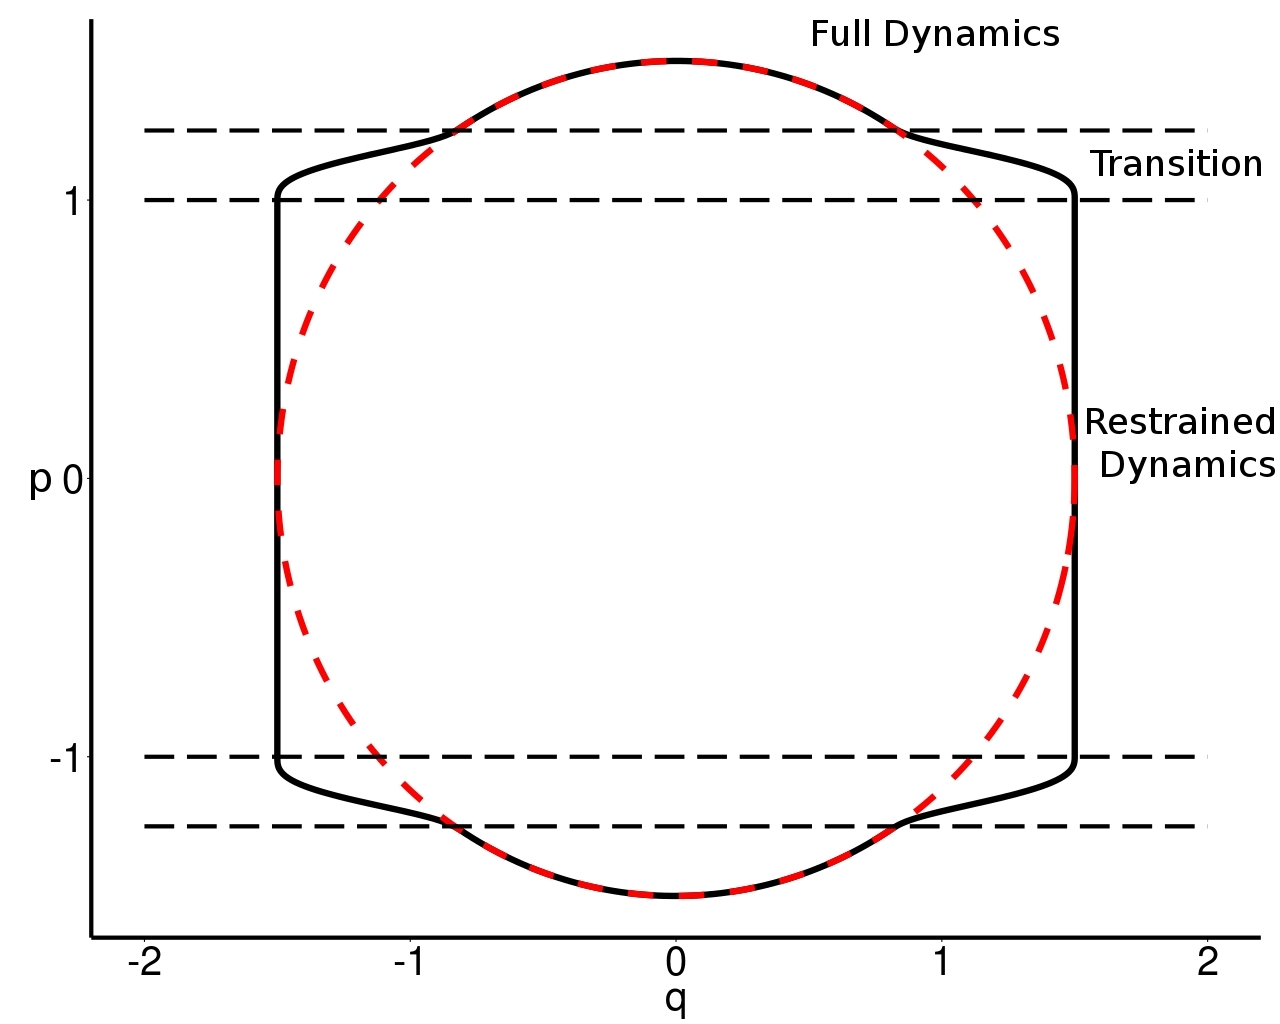
\includegraphics[width=1.0\linewidth]{images/arps-vriphys2013/harmonicOscillatorPhasePortraitraw.jpeg}
  \caption{\label{fig:harmonicOscillatorPhasePortrait} Phase portrait of a harmonic oscillator. The red dotted ellipse corresponds to standard Hamiltonian mechanics, while the solid black line corresponds to ARPS. During restrained dynamics momentum is accumulated. Then a transition deals with the accumulated energy before getting back to the full dynamics.}
\end{figure}
%-------------------------------------------------------------------------
\paragraph*{Computational performance:}
\cite{Artemova2012} obtained significant speedup exploiting immobility of particles.
An incremental method was used to update the particles forces at each time step, while saving time on inactive particles :
\begin{enumerate}
    \item All forces that were acting on each active particle at the previous time step are substracted based on previous position.
    \item New forces based on current positions are added to each active particle.
\end{enumerate}
%%%% MP: pasclair: pas d’update forces entre une active et une inactive?
The computational performance comes from the absence of force computation between
two inactive particles and the absence of neighbor search for inactive particles.
As these two steps are common bottlenecks in particle simulation, significant speedup were achieved.

%-------------------------------------------------------------------------
\paragraph*{Potential benefits of extension to Computer Graphics:}
Molecular dynamics often inspired particle-based simulations in Computer Graphics. The same bottleneck, namely inter-particles forces computation based on neighbor search, is present in the two fields, so we can expect interesting performance for ARPS in graphics. The remainder of this paper explores two applications of ARPS to graphical simulations:
\begin{enumerate}
\item Particle-based fluid simulation. In this case, damping forces are involved in contrast with the classic use of ARPS.
We propose a method to handle them as well as an incremental algorithm to update the forces and the scalar fields.
\item Stiff object simulation. We take the example of a cloth simulation.
We will propose an implicit formulation of ARPS and a hybrid solver to exploit inactivity of particles.
\end{enumerate}
It is clear that ARPS is not well-suited for simulations where all degree of freedom move: classical spatial adaptation is better suited in this case. In contrast, ARPS is best suited for simulations where most parts are immobile but may resume moving at any time. Even if these situations are not the most visually exciting, they are very common in Computer Graphics: they include simulation of characters clothing when many of the characters are at rest, surgical simulations with local user interaction, and the animation of large volumes of liquid, when most of it already came to rest.





%-------------------------------------------------------------------------
\section{ Extension to SPH fluid simulation } \label{sec sph}
SPH fluid simulation is widely used in computer graphics and many methods have been proposed \cite{Desbrun:1996:SPN}, \cite{Muller2003}, \cite{Solenthaler2009}, \cite{implicitSPH}.
SPH approximates fluid dynamics with a set of particles.
The particles are used to interpolate properties of the fluid anywhere in the space.
Each particle samples fluid properties such as density, pressure or temperature. All these properties are updated based on the particle neighbors and are
used in short-ranged inter-particle forces.
For a detailed and comprehensive introduction to SPH, you can refer to \cite{Monaghan2005}.
To integrate ARPS, we chose WCSPH (Weakly Compressible Smoothed Particle Simulation) \cite{Becker2007WCSPH}, a standard SPH formulation \cite{Desbrun:1996:SPN}, \cite{Muller2003}.
We limited our simulation to the main inter-particles forces: pressure and viscosity.
Classically a SPH algorithm follows three steps:
\begin{enumerate}
	\item Update mass density and pressure
	\item Compute inter-particles forces : pressure, viscosity
	\item Integrate velocities and positions
\end{enumerate}
With ARPS, time can be saved on each computation step involving pairwise terms.
In SPH, inter-particles forces and density field computation are the perfect candidates.
As proposed in \cite{Artemova2012}, we use an incremental algorithm to update only quantities involving active particles.
%-------------------------------------------------------------------------------
\subsection{Viscosity}
Viscosity forces involve particles velocities. The viscosity force of particle $i$ with respect to particle $j$ is :
\begin{equation}
	\label{eq:viscosityForces}
	f_{ij} =
	\left\lbrace	
	\begin{array}{lrr}
	-m_{i}m_{j}\Pi_{ij}\nabla W_{ij} & & v_{ij}^{T}q_{ij}<0\\
	& & \\
	0 & & v_{ij}^{T}q_{ij} \geq 0 \\
	\end{array}		
	\right.
\end{equation}
$\Pi_{ij}$ is given as :
\begin{equation}
\label{eq:pij}
	\Pi_{ij} = -\nu\left( \frac{v_{ij}^{T}q_{ij}}{ \mid q_{ij} \mid^{2} + \epsilon h^{2} } \right)
\end{equation}
$W_{ij}$ denotes a convolution kernel, $v_{ij}$ the difference of velocities between the two particles, $q_{ij}$ the difference of positions between the two particles, $m_{i}$ is the mass, $h$ is the particle smoothing radius and $\nu = \frac{2 \alpha h c_{s}}{ d_{i} + d_{j} }$ is a viscous term where $\alpha$ is a viscosity constant,
$d_{i}$ the particle $i$ density.
$\epsilon=0.01$ is a constant to avoid singularities.
\newline \newline
However, velocity is not explictly represented in ARPS, and can be seen in two different ways. We may define it based on the momentum and set $ v_{i} = p_{i} / m_{i} $, or based on the change of position $  \dot{q}_{i}$.
In the first case, we can get time-varying forces even for inactive particles, which we want to avoid.
We therefore use the effective velocity of the particle, as defined in eq.(\ref{eq:adaptiveVelocity}).
Applied to a harmonic oscillator, this results in the behavior illustrated in Fig. \ref{fig:HODampedPP}.
The more the particle is damped the longer it remains inactive, which is an intuitive behavior.
%%% HARMONIC OSCILLATOR DAMPED%%%
\begin{figure}[htb]
  \centering
  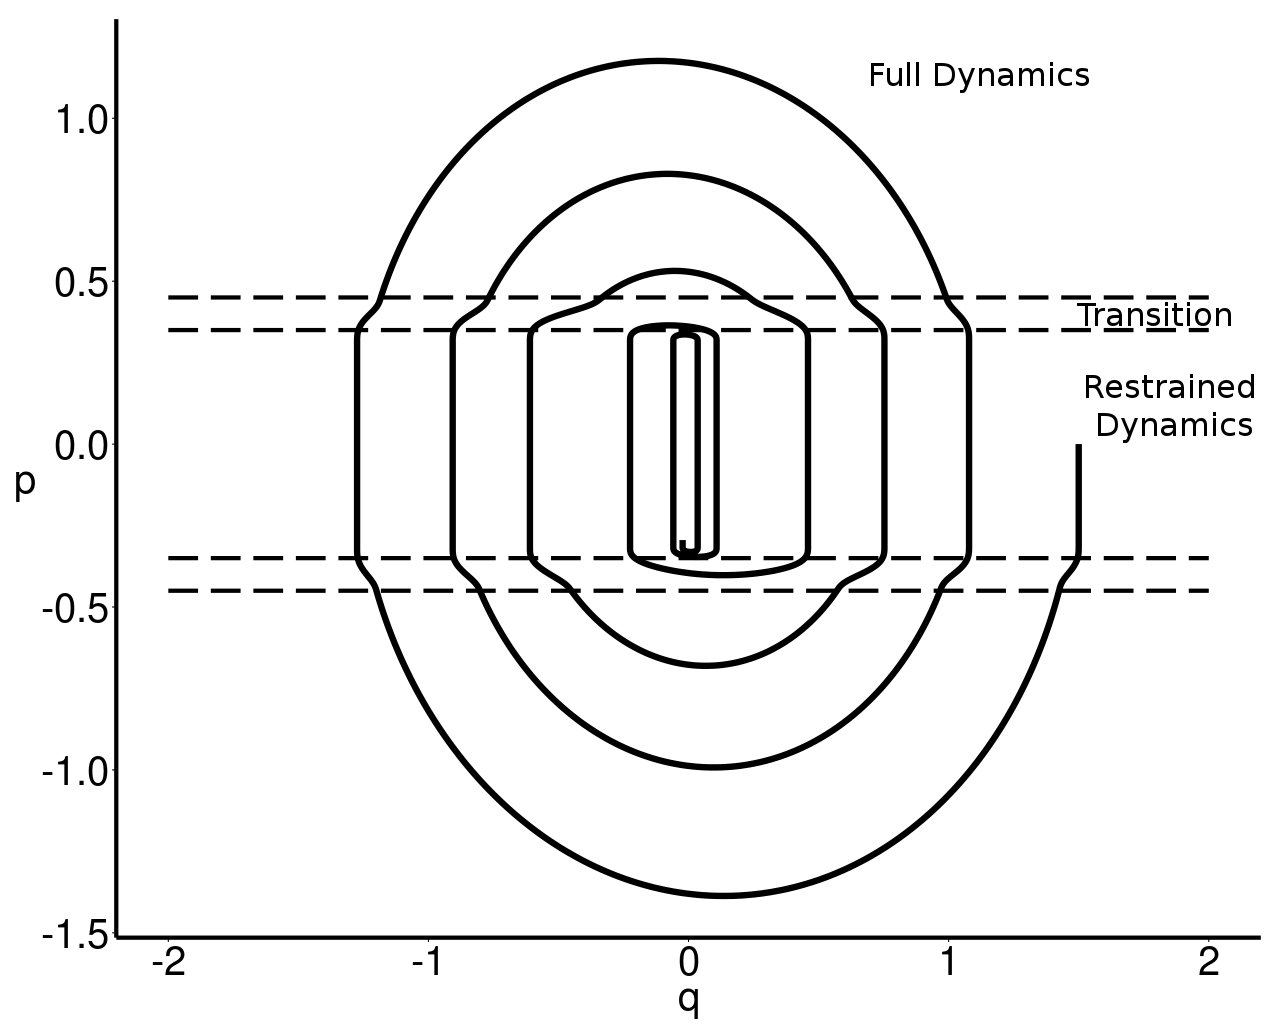
\includegraphics[width=1.0\linewidth]{images/arps-vriphys2013/harmonicOscillatorDampedPhasePortraitraw.jpeg}
  \caption{\label{fig:HODampedPP} Phase portrait of our damping approach in ARPS.
  As with a classic damped oscillator we obtain a spiral phase portrait.}
\end{figure}
%-------------------------------------------------------------------------
\subsection{Modified inactivity criterion}
Since our damping force vanishes along with the effective velocity of the particle, it drags down the kinetic energy asymptotically close to the inactivity threshold, without ever reaching it.
Consequently, particles only subject to damping forces never become inactive, and we do not spare computation time, even when the particles get nearly static.
To remedy this problem, we consider inactive the particles which effective velocity fall below a user-defined threshold.

% we introduce a new criterion which adaptively combines energy evaluation with position variation.
% The particle is set inactive if
% \begin{equation}
% 	\label{eq:convergence}
% 	\rho_i > 1 - \frac{\alpha m}{\rho h}
% \end{equation}
% where $\alpha$ is a user-defined constant.
% \TODO{Comment choisir $\alpha$.}
% %%% SPH-ARPS %%%
% \begin{figure}[htb]
%   \centering
%   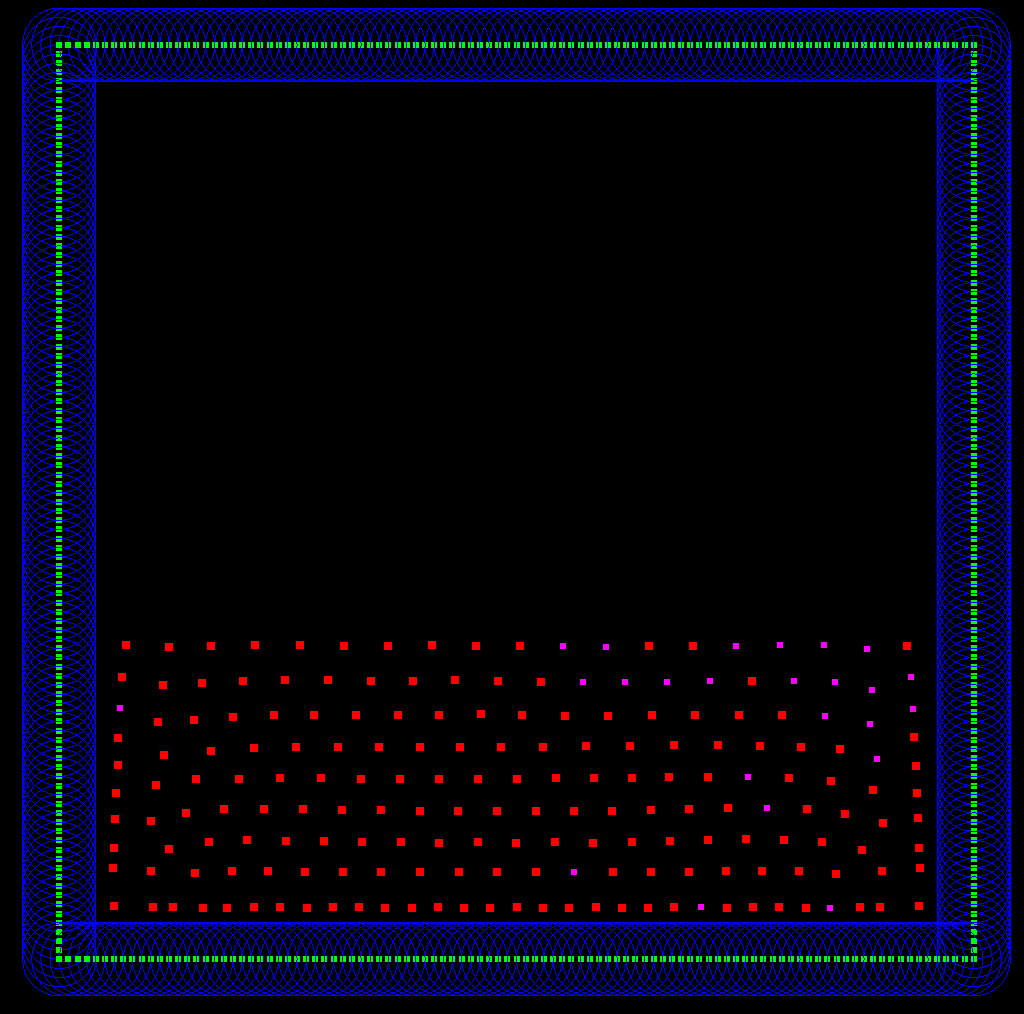
\includegraphics[width=.8\linewidth]{sphARPSraw.png}
%   \caption{\label{fig:sphARPS} Soon wonderful SPH application}
% \end{figure}
%\TOREWRITTEN{
%    Known limitations are the convergence near more inactive particles
%    and following the parameters the need to reduce time step to well take
%    transitions.
%}
%-------------------------------------------------------------------------
\subsection{Performance}
We performed two experiments to measure computation time.
The first one (Table~\ref{table:perf1}) is a fall of $5000$ particles in a box.
As soon as most particles come to rest, and become inactive the speedup can be significant.
For $15$s, the mean speedup is $3.8$.
The speedup can locally reach $25.7$.
%\begin{table}[htb]
%   \centering
%\begin{tabular}{|c|c|c|c|} \hline
%    Simulation Time & SPH   & SPH + ARPS    & Speed-up \\ \hline
%            15s     & 893   & 232s          &  3.8x\\ \hline
%            30s     & 1814 & 269s           &  6.7x\\ \hline
%\end{tabular}
%\caption{\label{table:perf1}Fall of a block of water - Computation time for different simulation times.}
%\end{table}
\begin{table}[htb]
   \centering
\begin{tabular}{|c|c|c|c|} \hline
    Simulation Time & SPH   & ARPS    & Speed-up \\ \hline
    15s     & 893s   & 232s                 &  \{0.91, 25.73, 3.85\}\\ \hline
\end{tabular}
\caption{\label{table:perf1}Fall of a block of water - Computation time and speedup \{min, max, mean\}}
\end{table}
We can see in Figure~\ref{fig:teaser} that during speed movements most of the particles are active so that the adaptive simulation stay close to reference simulation.
Therefore small scale details like splashes can be preserved.
\begin{figure*}[!ht]
    \centering
    \begin{tabular}{ccc}
        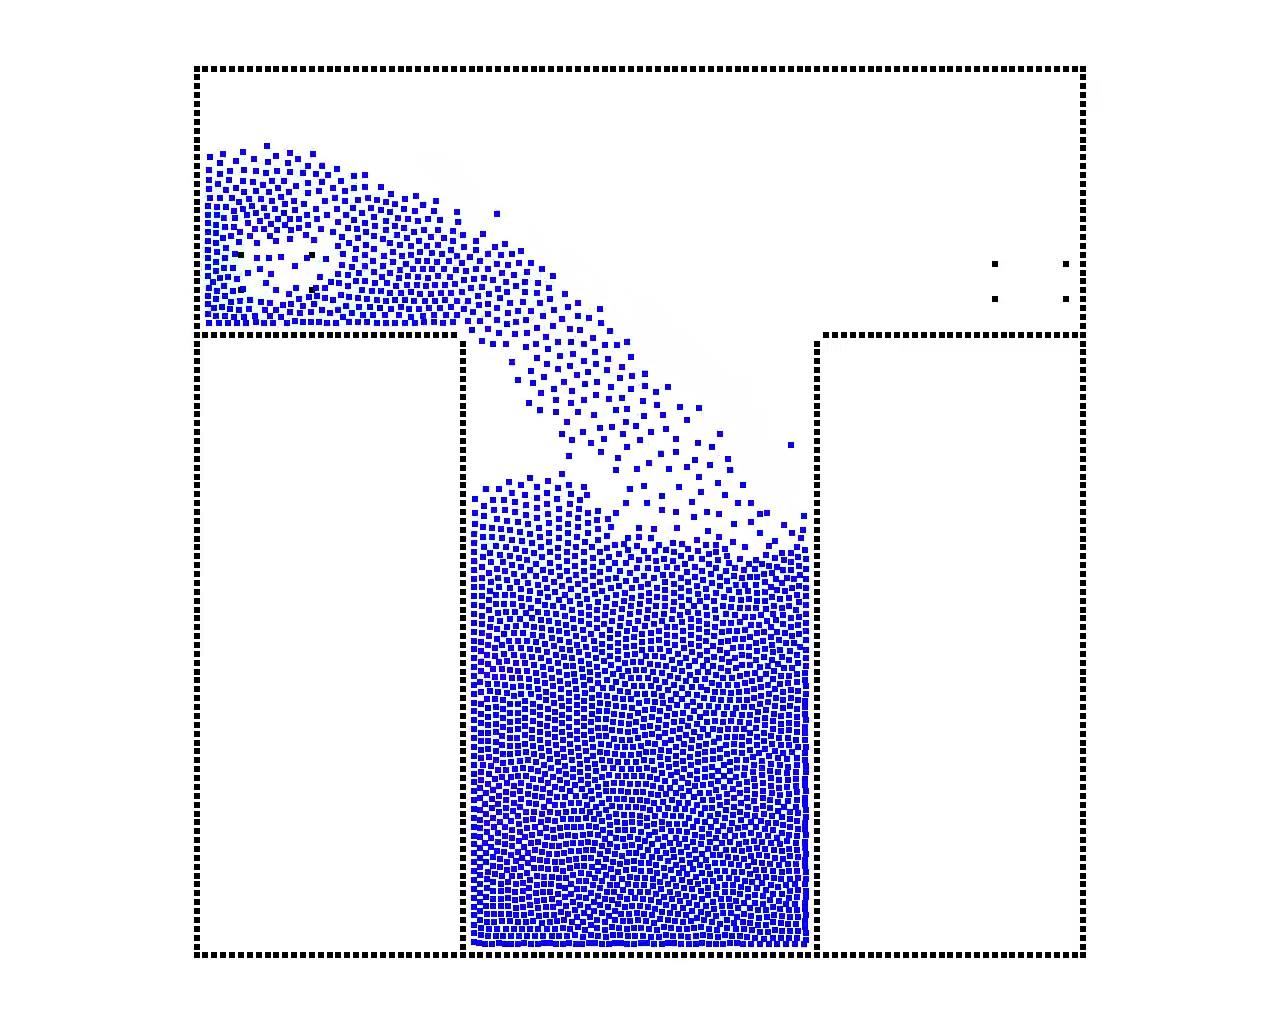
\includegraphics[width=.32\linewidth]{images/arps-vriphys2013/PermanentFlowSPH.jpg} &
        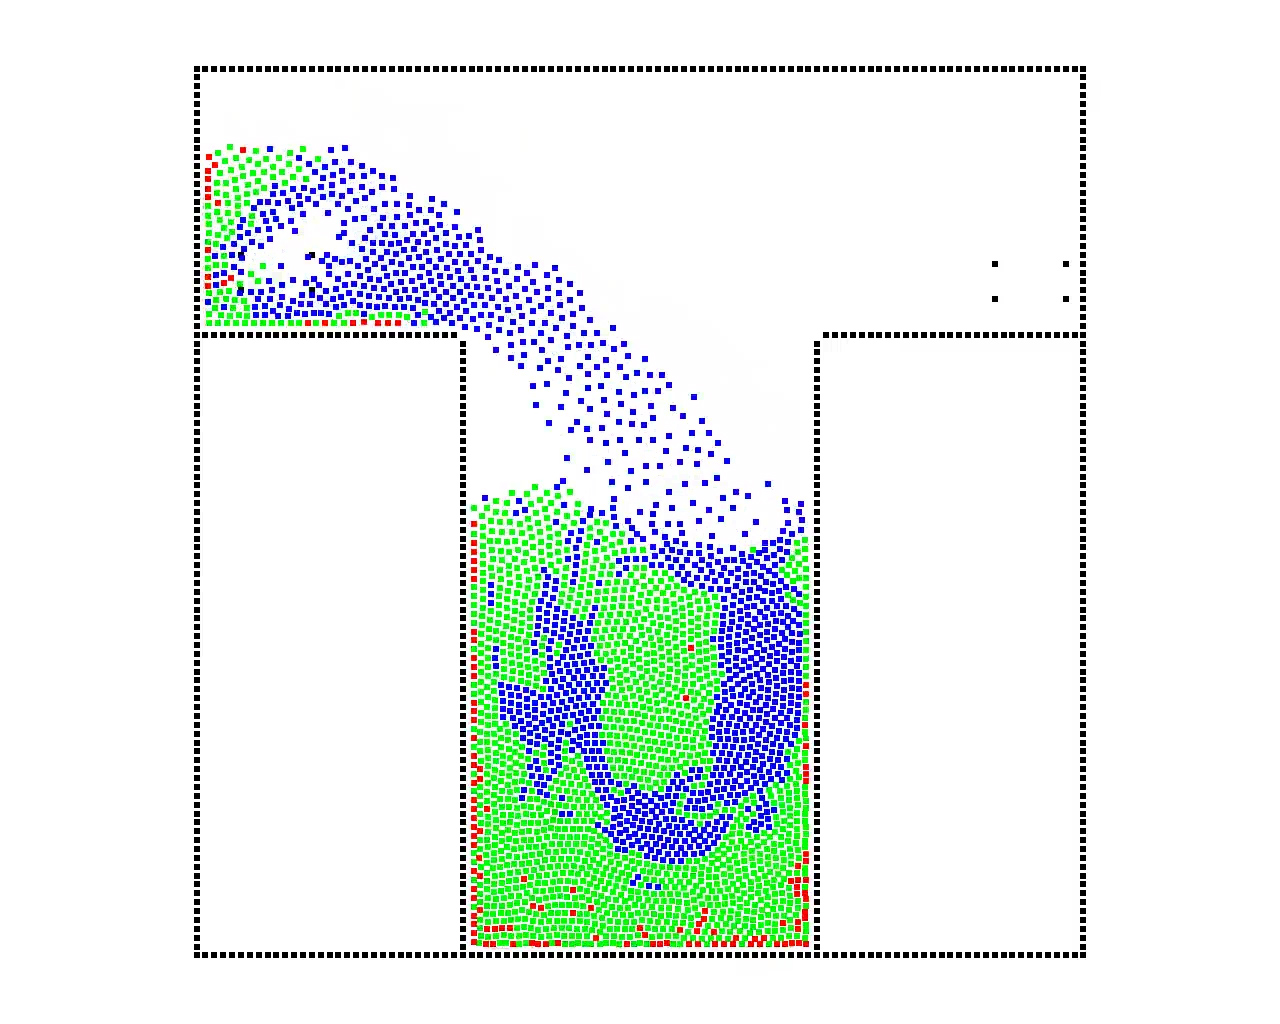
\includegraphics[width=.32\linewidth]{images/arps-vriphys2013/PermanentFlowARPSColor.jpg} &
  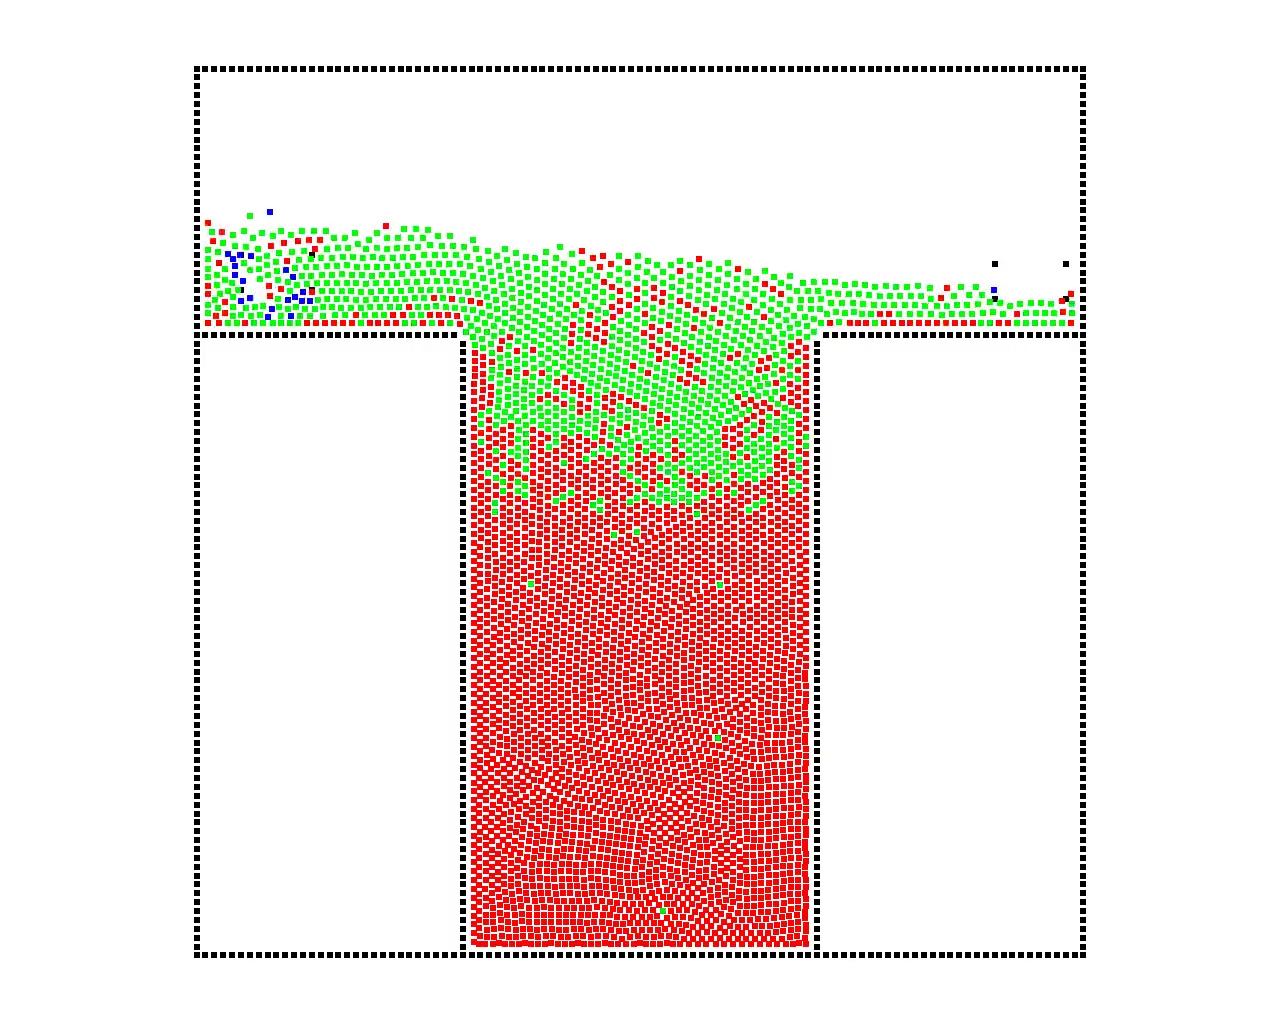
\includegraphics[width=.32\linewidth]{images/arps-vriphys2013/PermanentFlowARPSColor2.jpg} \\
  (a) & (b) & (c)
    \end{tabular}
    \caption{\label{fig:permanentflow} A permanent flow simulation with 4240 particles.
    (a) is a classic WCSPH simulation. (b) is our adaptive method at the same time of (a) with restrained particles in red. (c) is our adaptive method once the permanent flow is installed.}
\end{figure*}
\newline
The second experiment (see Table~\ref{table:perf2}) is the creation of a permanent flow with $4240$ particles. As we can see in Figure~\ref{fig:permanentflow}, once the permanent flow is installed a large amount of particles are restrained. We reach an interesting speedup while keeping a motion close to the reference.
%\begin{table}[htb]
%    \centering
%\begin{tabular}{|c|c|c|c|} \hline
%    Simulation Time & SPH       & SPH + ARPS    & Speed-up \\ \hline
%        30s         & 2166s     & 814s          & 2.7x \\ \hline
%        60s         & 4596s     & 1571          & 2.9x \\ \hline
%\end{tabular}
%    \caption{\label{table:perf2}Fluid permanent flow - Computation time for different simulation times.}
%\end{table}
\begin{table}[htb]
    \centering
\begin{tabular}{|c|c|c|c|} \hline
    Simulation Time & SPH       & ARPS    & Speed-up \\ \hline
    30s         & 2166s     & 814s              & \{0.83, 3.99, 2.66\} \\ \hline
\end{tabular}
\caption{\label{table:perf2}Fluid permanent flow - Computation time and speedup \{min, max, mean\}.}
\end{table}
%-------------------------------------------------------------------------
\section{Extension to stiff objects: Implicit Integration} \label{sec cloth}
In this section we explore the application of ARPS to stiff object simulation and propose an implicit integration scheme which saves computation time for particles at rest.
%------------------------------------------------------------------------
% \subsection{Limitations of explicit integration for computer graphics }
% In stiff object simulation bottle-necks completely change.
% We generally know the topology of the object so we do not have neighbor search to perform.
% Because of stiff equations of motion, a small time step must be used to keep a stable simulation.
% These two differences displace the bottle-neck from interp-articles force computation to time integration.
% In simulation where high spatial resolution is requested, it implies important computational cost.
% A common solution, especially in the field of cloth simulation, is to use an implicit integration scheme instead of an explicit one.
% Thus large time steps can be handled.
%------------------------------------------------------------------------
Implicit integration for cloth simulation was introduced in \cite{Baraff1998}. An introduction to implicit integration is proposed in \cite{Witkin2001}.
While originally formulated on velocity, it can be straightforwardly expressed on momentum.
Instead of integrating the momentum using the forces at the current time step, implicit integration uses the forces at the end of the current step.
As we do not know these forces we end up with a non linear function and after linearization with a linear system to solve to obtain the next momentum:
\begin{equation}
    \label{eq:implicit}
    ( I -h^{2}KM^{-1} ) \Delta p = h( f + h KM^{-1}p ) \;,
\end{equation}
where $\displaystyle K = \frac{\partial f}{ \partial q}$ is the stiffness matrix and
$M$ is the mass matrix.
Solving the linear system is more costly than explicit integration, but it allows the use of larger time steps without any loss of stability, enabling to advance much faster.
%------------------------------------------------------------------------
\subsection{ ARPS Implicit Integration }
We derive an implicit integration scheme from Adaptively Restrained equations of motion.
The linear system has to take into account the state of the particles.
The discrete equations of motions for implicit Euler are:
\begin{equation}
	\label{eq:implicitEqMotion}
	\begin{array}{l}
	\displaystyle \Delta p =  h f(q_{n+1}, p_{n+1})\\
				\\
	\displaystyle \Delta q = h \left( M^{-1}(1-\rho(p_{n+1}))p_{n+1} \right. \\
	\displaystyle \left. - \frac{1}{2	}p_{n+1}^{T} M^{-1} \frac{\partial \rho(p_{n+1})}{\partial p}p_{n+1} \right)
	\end{array}
\end{equation}
We perform a Taylor-Young expansion of $f(q_{n+1}, p_{n+1})$ and introduce $\Delta q$ in the expended momenta equation.
We then perform a Taylor-Young expansion of $\rho(p_{n+1})$ in the momentum equation, which gives us the following equation system:
\begin{equation}
	\label{eq:arpsLinearSystem}
	( I -h^{2}KRM^{-1} ) \Delta p = h( f + h KM^{-1}s )
\end{equation}
$R$ is a block-diagonal matrix where each $3\times 3$ block $R_{ii}$ is:
\begin{equation}
	\label{eq:Ri}
	\begin{array}{l}
	\displaystyle R_{ii} = I - \rho(p^{i}_{n}) - p^{i}_{n} \frac{\partial \rho(p^{i}_{n})}{\partial p_{i}}^{T} \\
	\displaystyle - \frac{1}{2}p^{i}_{n}p^{i^{T}}_{n}\frac{\partial^{2} \rho(p^{i}_{n})}{\partial p_{i}^{2}}^{T} -
	\displaystyle \frac{\partial \rho(p^{i}_{n})}{\partial p_{i}} p^{i^{T}}_{n} \;,
	\end{array}
\end{equation}
while $s$ is a $3N$ vector where $N$ is the number of particles, and each $s_{i}$ is :
\begin{equation}
	\label{eq:si}
	\displaystyle s_{i} = p^{i}_{n} - \rho(p^{i}_{n})p^{i}_{n} - \frac{1}{2	}p^{i^{T}}_{n}p^{i}_{n}\frac{\partial \rho(p^{i}_{n})}{\partial p_{i}}
\end{equation}
Note that if all particles are inactive then we have $R = 0$ and $s = 0$ and we get an explicit formulation:
\begin{equation}
    \label{eq:ARPSImplicitRestrained}
    I \Delta p = h f
\end{equation}
Conversely, if all particles are active then $R = I$ and $s = p$ and we get the classical implicit formulation of eq.(\ref{eq:implicit}).
We loop over time using algorithm \ref{alg:ARPSimplicit}.
\begin{algorithm}[H]
    \caption{Implicit integration scheme}
    \label{alg:ARPSimplicit}
    \begin{algorithmic}[10]
	\For{ each time step}
	    \State compute $\rho, R, s, f$.
	    \State compute $A = I - h^{2}KRM^{-1}$
	    \State compute $b = h f + h^{2}KM^{-1}s$
	    \State solve $A \Delta p = b$
            \State compute $p_{n+1} = p_{n} + \Delta p$
	    \State compute $\displaystyle q_{n+1} = q_{n} +
            hM^{-1}\left( R\Delta p+ s \right)$
	\EndFor
    \end{algorithmic}
\end{algorithm}
\begin{figure}[htb]
  \centering
  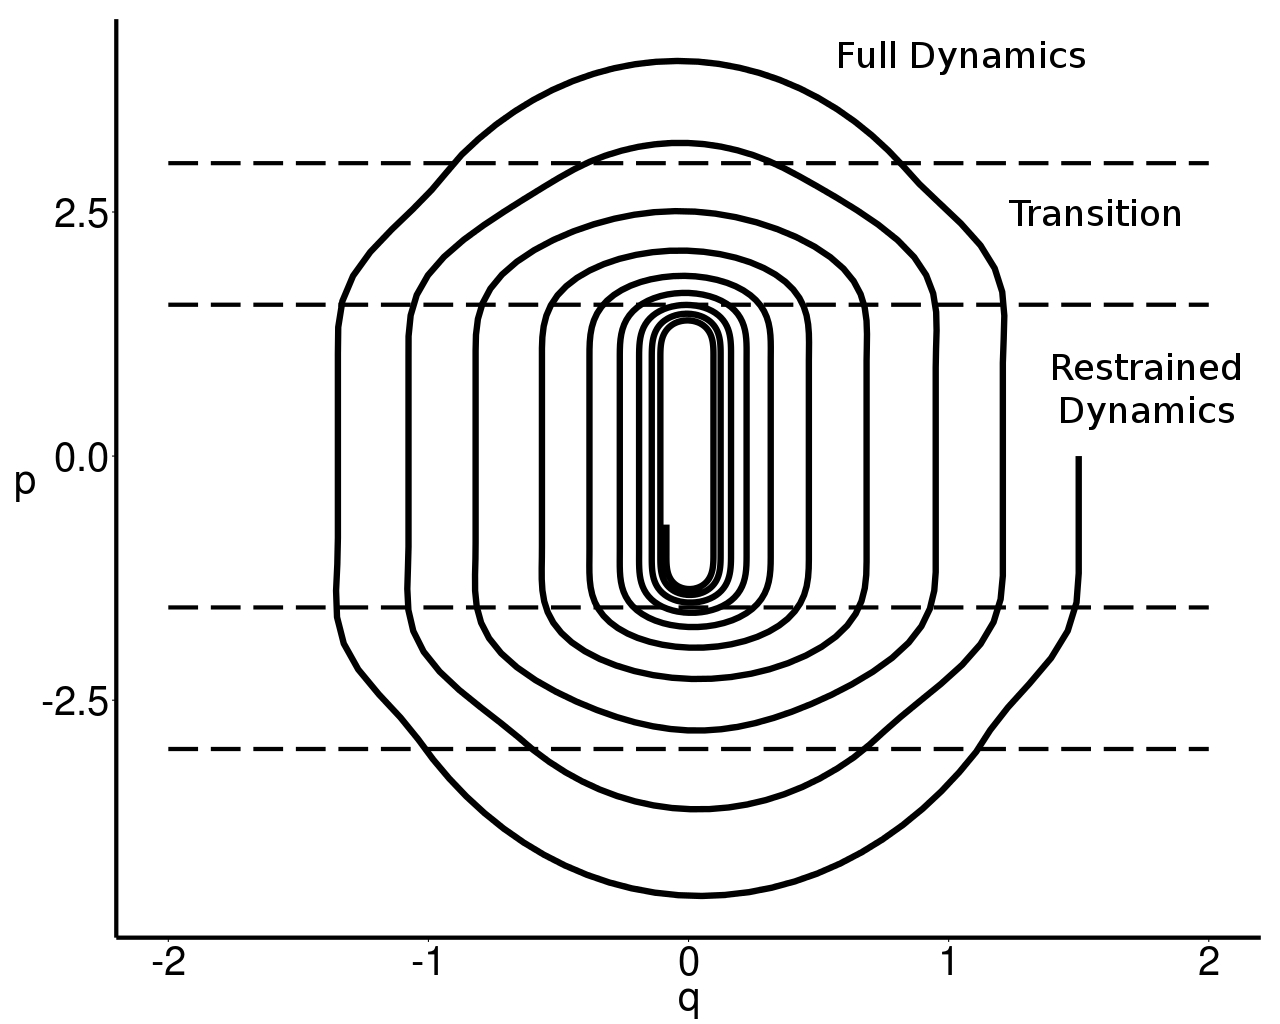
\includegraphics[width=1.0\linewidth]{images/arps-vriphys2013/implicitHOPPraw.jpeg}
  \caption{\label{fig:implicitHOPP} Phase portrait of a harmonic oscillator simulated using implicit ARPS.}
\end{figure}

Figure~\ref{fig:implicitHOPP} shows the phase portrait of a harmonic oscillator simulated using our implicit formulation.
As expected, the well-known numerical damping effect of implicit Euler provides us with the same behavior we could observe with a damped harmonic oscillator.
%%% IMPLICIT HARMONIC OSCILLATOR DAMPED%%%
To include a damping term in the physical model, we derived an implicit formulation which includes a damping term $f_{d} = -\gamma \dot{q}$:
\begin{equation}
	\label{eq:arpsLinearSystemDamped}
	( I + h\gamma M^{-1}R -h^{2}KRM^{-1} ) \Delta p = h( f + h KM^{-1}s + f_{d})
\end{equation}
%\begin{algorithm}[H]
%    \caption{Implicit integration scheme with damping $f_{damping}=-\gamma \dot{q}$}
%    \label{alg:ARPSimplicitDamped}
%    \begin{algorithmic}[10]
%	\For{ each time step}
%	    \State compute $\rho, R, s, f$.
%            \State compute $A = I + h\gamma M^{-1}R - h^{2}KRM^{-1}$
%            \State compute $b = h ( f + f_{damping} ) + h^{2}KM^{-1}s $
%	    \State solve $A \Delta p = b$
%            \State compute $p_{n+1} = p_{n} + \Delta p$
%	    \State compute $\displaystyle q_{n+1} = q_{n} +
%            hM^{-1}\left( R\Delta p+ s \right)$
%	\EndFor
%    \end{algorithmic}
%\end{algorithm}
%\TOREWRITTEN{We add adaptive artificial damping.}
%\newline
%\TOREWRITTEN{Need to reformulate the position update (Taylor Young)}
%------------------------------------------------------------------------
\paragraph*{Solving the equation:}
We exploit inactive particles to save computation time.
As discussed earlier, inactive particles can be handled using explicit integration, which is much simpler.
When a particle is inactive and has no active neighbors we do not need to include it in the linear system.
We thus build the minimal linear system, which only contains active particles and their neighbors.
These particles are implicitly integrated, while the others are explicitly integrated.
%\begin{table}[htb]
%    \centering
%\begin{tabular}{|c|c|c|c|} \hline
%    Simulation Time & Implicit & Hybrid & Speed-up \\ \hline
%            20s     & 16.9s               & 6.2s            &  2.7x\\ \hline
%            40s     & 32.1s               & 6.5s            &  4.9x\\ \hline
%            80s     & 62.5s               & 8.8s            &  7.1x\\ \hline
%\end{tabular}
%    \caption{\label{tab:clothePerf}Implicit solver vs Hybrid solver. Computation time for different simulation times.}
%\end{table}
\begin{table}[htb]
    \centering
\begin{tabular}{|c|c|c|c|} \hline
    Simulation & Implicit  & Hybrid    & Speed-up \\
    Time & & & \\ \hline
    20s             & 16.9s     & 6.2s      &  \{0.77, 15.16, 2.73\}\\ \hline
\end{tabular}
\caption{\label{tab:clothePerf}Implicit solver vs Hybrid solver. Computation time and speedup \{min, max, mean\}.}
\end{table}
%\TODO{Il faut que je relance ces calculs car SOFA bloquait les performances pour l'affichage,
%mais je ne m'attend pas à un gros speedup, je trouve ça très surprenant et je ne vois pas d'où
%ça peut venir à part de l'implémentation.}
Figure~\ref{fig:clothARPS} shows a hanging cloth with active and inactive particles.
At the beginning all the particles become active. Then a moving front of inactivation/reactivation traverses the cloth at decreasing frequency. The cloth finally finds a rest position, where all the particles are inactive and simulated explicitly, saving computation time. The particles can become active again if external forces or imposed motion are applied.
\begin{figure}[htb]
  \centering
  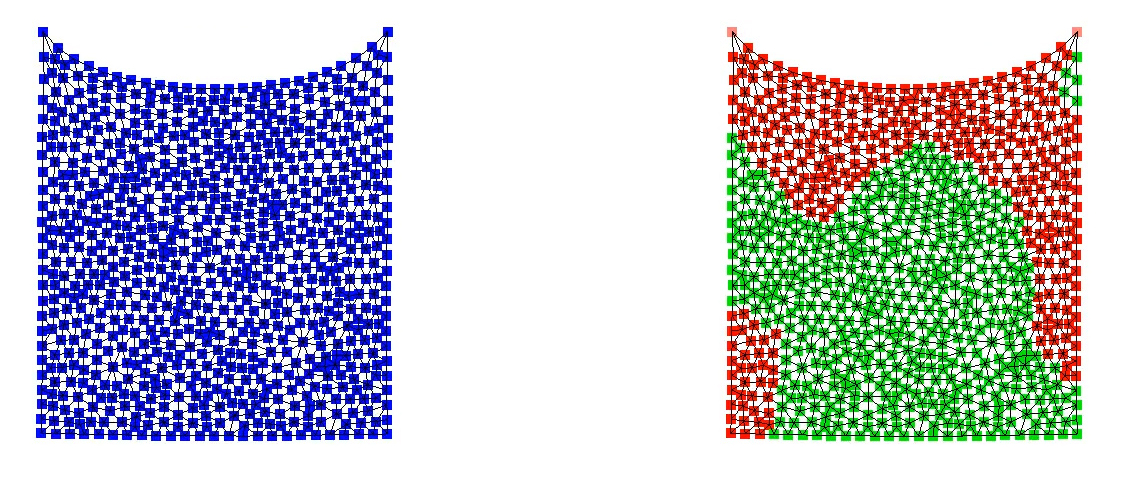
\includegraphics[width=1.0\linewidth]{images/arps-vriphys2013/Square3.jpg}
  \caption{\label{fig:clothARPS} Hanging cloth. Left: traditional implicit simulation. Right: implicit ARPS simulation with a varying set of active and inactive particles. }
\end{figure}
Table~\ref{tab:clothePerf} shows performances we achieved with our hybrid solver.
As soon as a large number of particles become inactive the simulation is explicitly integrated and interesting speedup can raise.
\newline
However, while smoothly varying external forces are well handled by our simulator, we noticed instabilities when interacting strongly with the model.
They seem to occur during the transition between the transitive and the full-dynamics states.
A more thorough study of the influence of the transition function $\rho$ on the stability of the system would be necessary to come up with robust implicit ARPS simulations.
 This transition should be really well taken to avoid any instabilities.
% Indeed if the transition is roughly taken and worse, jumped, it will results in a position discontinuities from a time step to another and creates instabilities.
% A solution we did not implemented yet would be to use an adaptive time step when a particle encounters the transition.
% It seems that the choice of the restraining function and the choice criterion have responsibilities in the simulation stability.
% We tested different restraining functions and stability results were really different.
% More precisely the second derivatives of the restraining function have a major role.
% We tested a straight restraining function, so no second derivatives, and less instabilities
% occurred.
%\QUESTION{Begin to talk more about the parameters of ARPS}
%------------------------------------------------------------------------


\section{Implementation} \label{sec implementation}
%\IDEA{
%\newline
%Discuter les deux parametres de lARPS -  vers quelles parametres tend on
%\newline
%Discuter la fonction de restriction : je ne sais pas comment
%\newline
%! Justifier l absence de resultats !
%\newline
%Deux mots sur le solver
%}
%-------------------------------------------------------------------------
\subsection{ Parameters }
ARPS use two parameters, $\epsilon^{r}$ and $\epsilon^{f}$ of Equation~\ref{eq:restrainingfunction}.
The main goal of ARPS in computer graphics is to save time when nothing happens.
So we generally want a low $\epsilon^{r}$ not to miss interesting movements.
When sudden movements occur, we want a normal reaction, so we want the inactive particles to quickly become active.
This requires a short transition, \textit{i.e.} $\epsilon^{f}$ close enough to $\epsilon^{r}$.
However, due to discrete time integration, a short transition may be stepped over, or not enough sampled, which may result in instabilities.
Currently we manually set the parameters, and defer the automatic tuning to future work.
In table \ref{tab:parameters} we refer the thresholds used in our simulations.
\begin{table}[htb]
    \centering
    \begin{tabular}{|c|c|c|c|} \hline
                & $\epsilon^{r}$    & $\epsilon^{f}$ & Tolerance \\ \hline
        SPH     &   1-e6            & 2-e5          & 8e-5 \\ \hline
        Cloth  &   0.05            & 1             & 1e-4 \\ \hline
\end{tabular}
    \caption{\label{tab:parameters} ARPS thresholds for SPH and Cloth simulation}
\end{table}

\subsection{Linear solver}
A linear equation solver is necessary in implicit integration, as presented in Section~\ref{sec cloth}.
In contrast with most formulations, implicit ARPS generally results in an unsymmetrical equation matrix, due to the matrix products in eq.(\ref{eq:arpsLinearSystem}).
We currently use a sparse LU solver from umfpack library, but it would be interesting to try a Conjugate Gradient method for unsymmetrical matrices to control the computation time, as it is usually done in implicit integration.

%-------------------------------------------------------------------------
\subsection{Choice of the restraining function and criterion}
In ARPS the restraining function is a $5^{th}$-order spline.
The spline directly depends on particle kinetic energy which is the \emph{restraining} criterion.
The implicit solver involves second derivatives of the restraining function, which may have large values, leading to instabilities.
We found that controlling the state of the particles based on momenta norm rather than kinetic energies seems to mitigate this and lead to more stable simulations.
We plan to investigate this issue in future work.


%-------------------------------------------------------------------------
\section{Discussion and concluding remarks} \label{sec discussion}
We have shown that ARPS, a new, simple approach to adaptive simulation, can effectively be applied to Computer Graphics, and we have demonstrated two specific applications.
The most successful one is the SPH simulation, for which we have obtained significant speedups with only minor changes to the original simulation method.
In the case of stiff material, we have obtained promising results for implicit integration, and we will address stability issues in future work, starting with a careful study of the restraining function.

Another interesting avenue is to employ non-physically-based transition criteria. The current one, based on kinetic energy, is well adapted to molecular dynamics simulation. In Computer Graphics, however, we are more interested in visual results. In future work, we thus plan to investigate the tuning of the transition thresholds based on visibility or distance to the camera, to even more focus the computational power where it most contributes to the quality of the result.

\chapter{Frame-based cutting}


%%%%%%%%%%%%%%%%%%%%%%%%%%%%%%%%%%%%%%%%%%%%%%%%

In this paper we propose a method for the interactive detailed cutting of deformable thin sheets. Our method builds on the ability of frame-based simulation to solve for dynamics using very few control frames while embedding highly detailed geometry - here an adaptive mesh that accurately represents the cut boundaries.
Our solution relies on a non-manifold grid to compute shape functions that faithfully adapt to the topological changes occurring while cutting.  New frames are dynamically inserted to describe new regions. We provide incremental mechanisms for updating simulation data, enabling us to achieve interactive rates. We illustrate our method with examples inspired by the traditional Kirigami artform.

%%%%%%%%%%%%%%%%%%%%%%%%%%%%%%%%%%%%%%%%%%%%%%%%%%%%%%%%%%%%%%%%
%                       INTRODUCTION
%%%%%%%%%%%%%%%%%%%%%%%%%%%%%%%%%%%%%%%%%%%%%%%%%%%%%%%%%%%%%%%%
\section{Introduction}

Over the last three decades, physics-based animation methods have been proposed to simulate a wide range of phenomena. Substantial progress has been achieved in terms of efficiency and realism.  
As a result, physics-based animation has found applications in film, games, craft, teaching, and training.

Combining interactive user actions and detailed convincing animations is crucial for user experience in simulation and games. Unfortunately, computational contraints limit the 
fidelity that can be achieved with physics-based animation
in interactive simulations. Often, the simulated objects lack detail compared to the rest of the virtual environment.
Furthermore, operations that modify the structure of the simulated objects, such as cutting, 
maybe incompatible with faster simulation methods.
When not prohibited, the latter generally exhibit strong limitations. Indeed, the level of sampling of a physically-based model usually depends on geometric complexity. Detailed cuts result in an increase of the sampling which directly impacts the performance. In practice, the number of samples is limited to ensure real-time performance. This limitation quickly prevents the user from applying detailed cuts.  

In this work, we address the issue of enabling detailed cuts at interactive rates in  thin sheets of deformable materials. Our method is able to capture detailed cuts while using a relatively low number of control nodes for the physically-based model.
Our approach to decoupling the samplings of the physical geometric models, is to use a mesh-less simulation method called the frame-based model \cite{Gilles2011}. In this method, the deformation field induced by animated frames is applied to the geometric model using skinning weights. As each frame can cover a large, detailed shaped region of the geometric mesh, only a few of them are typically required.

\begin{figure}[t]
\centering
\begin{subfigure}[b]{0.45\linewidth}
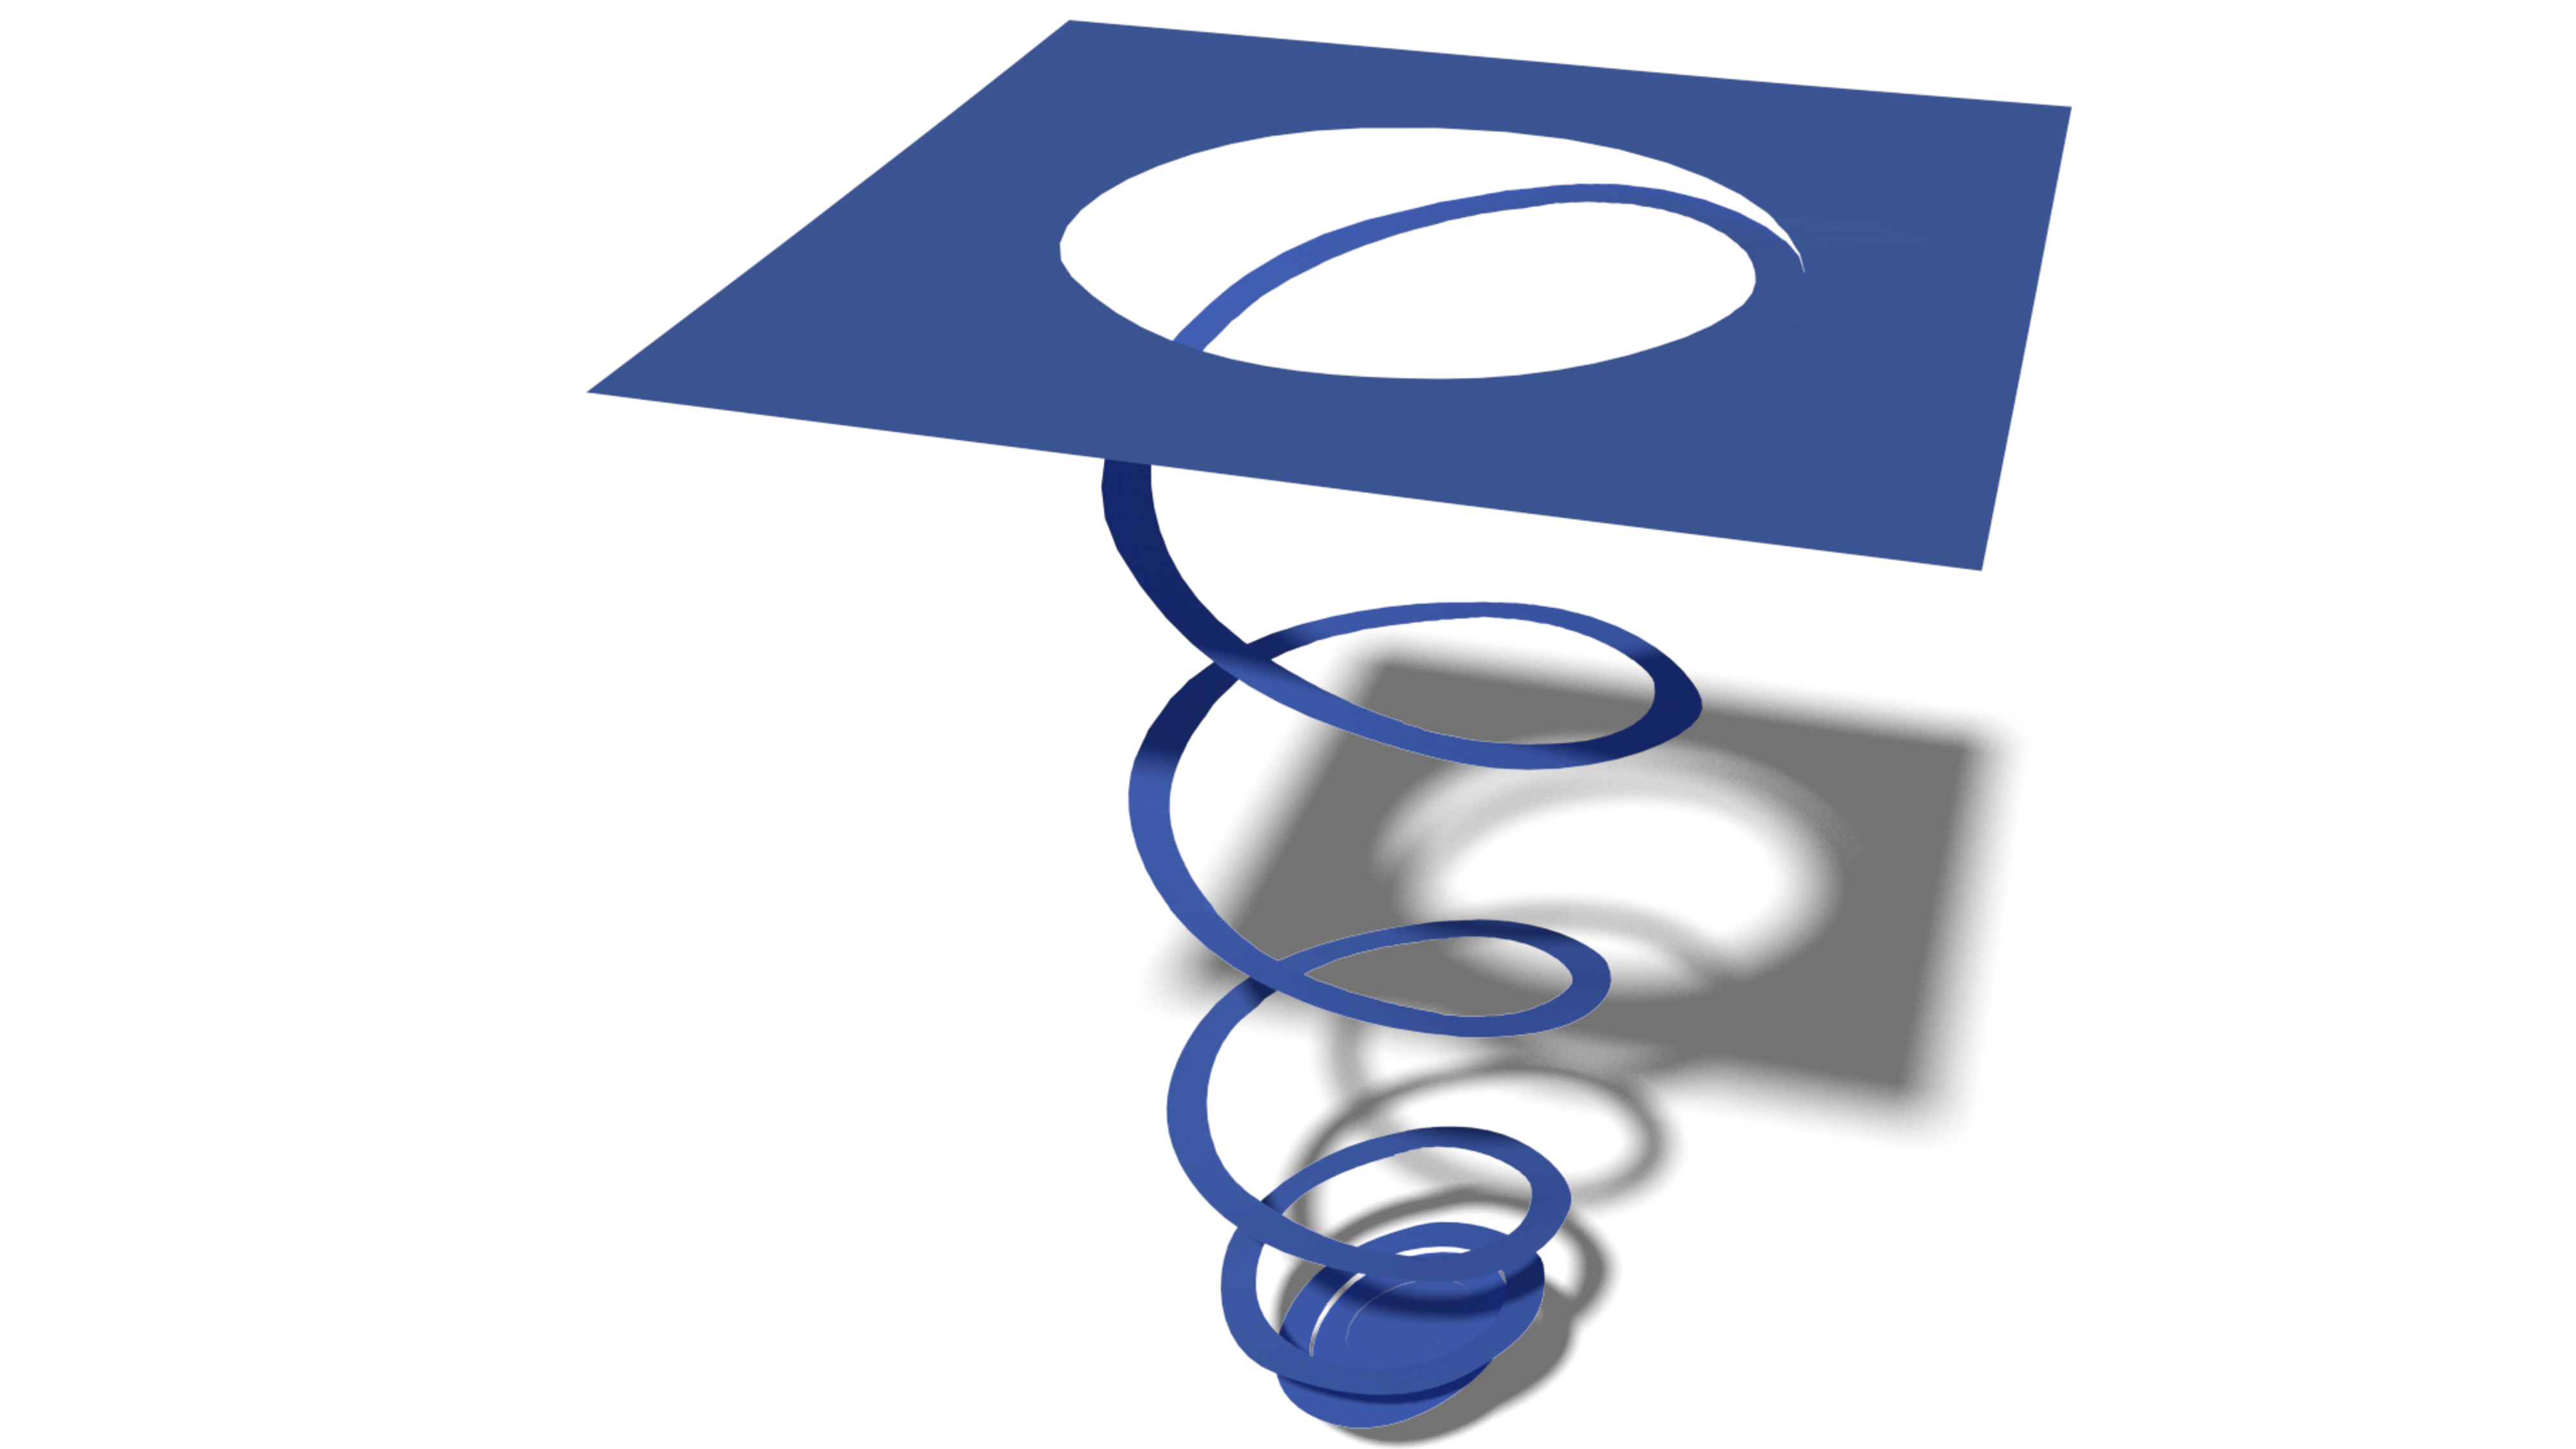
\includegraphics[width=\linewidth]{images/cutting-mig2015/Spiral2.pdf}
\caption{\label{fig:spiral}}
\end{subfigure}
\hfill
\begin{subfigure}[b]{0.45\linewidth}
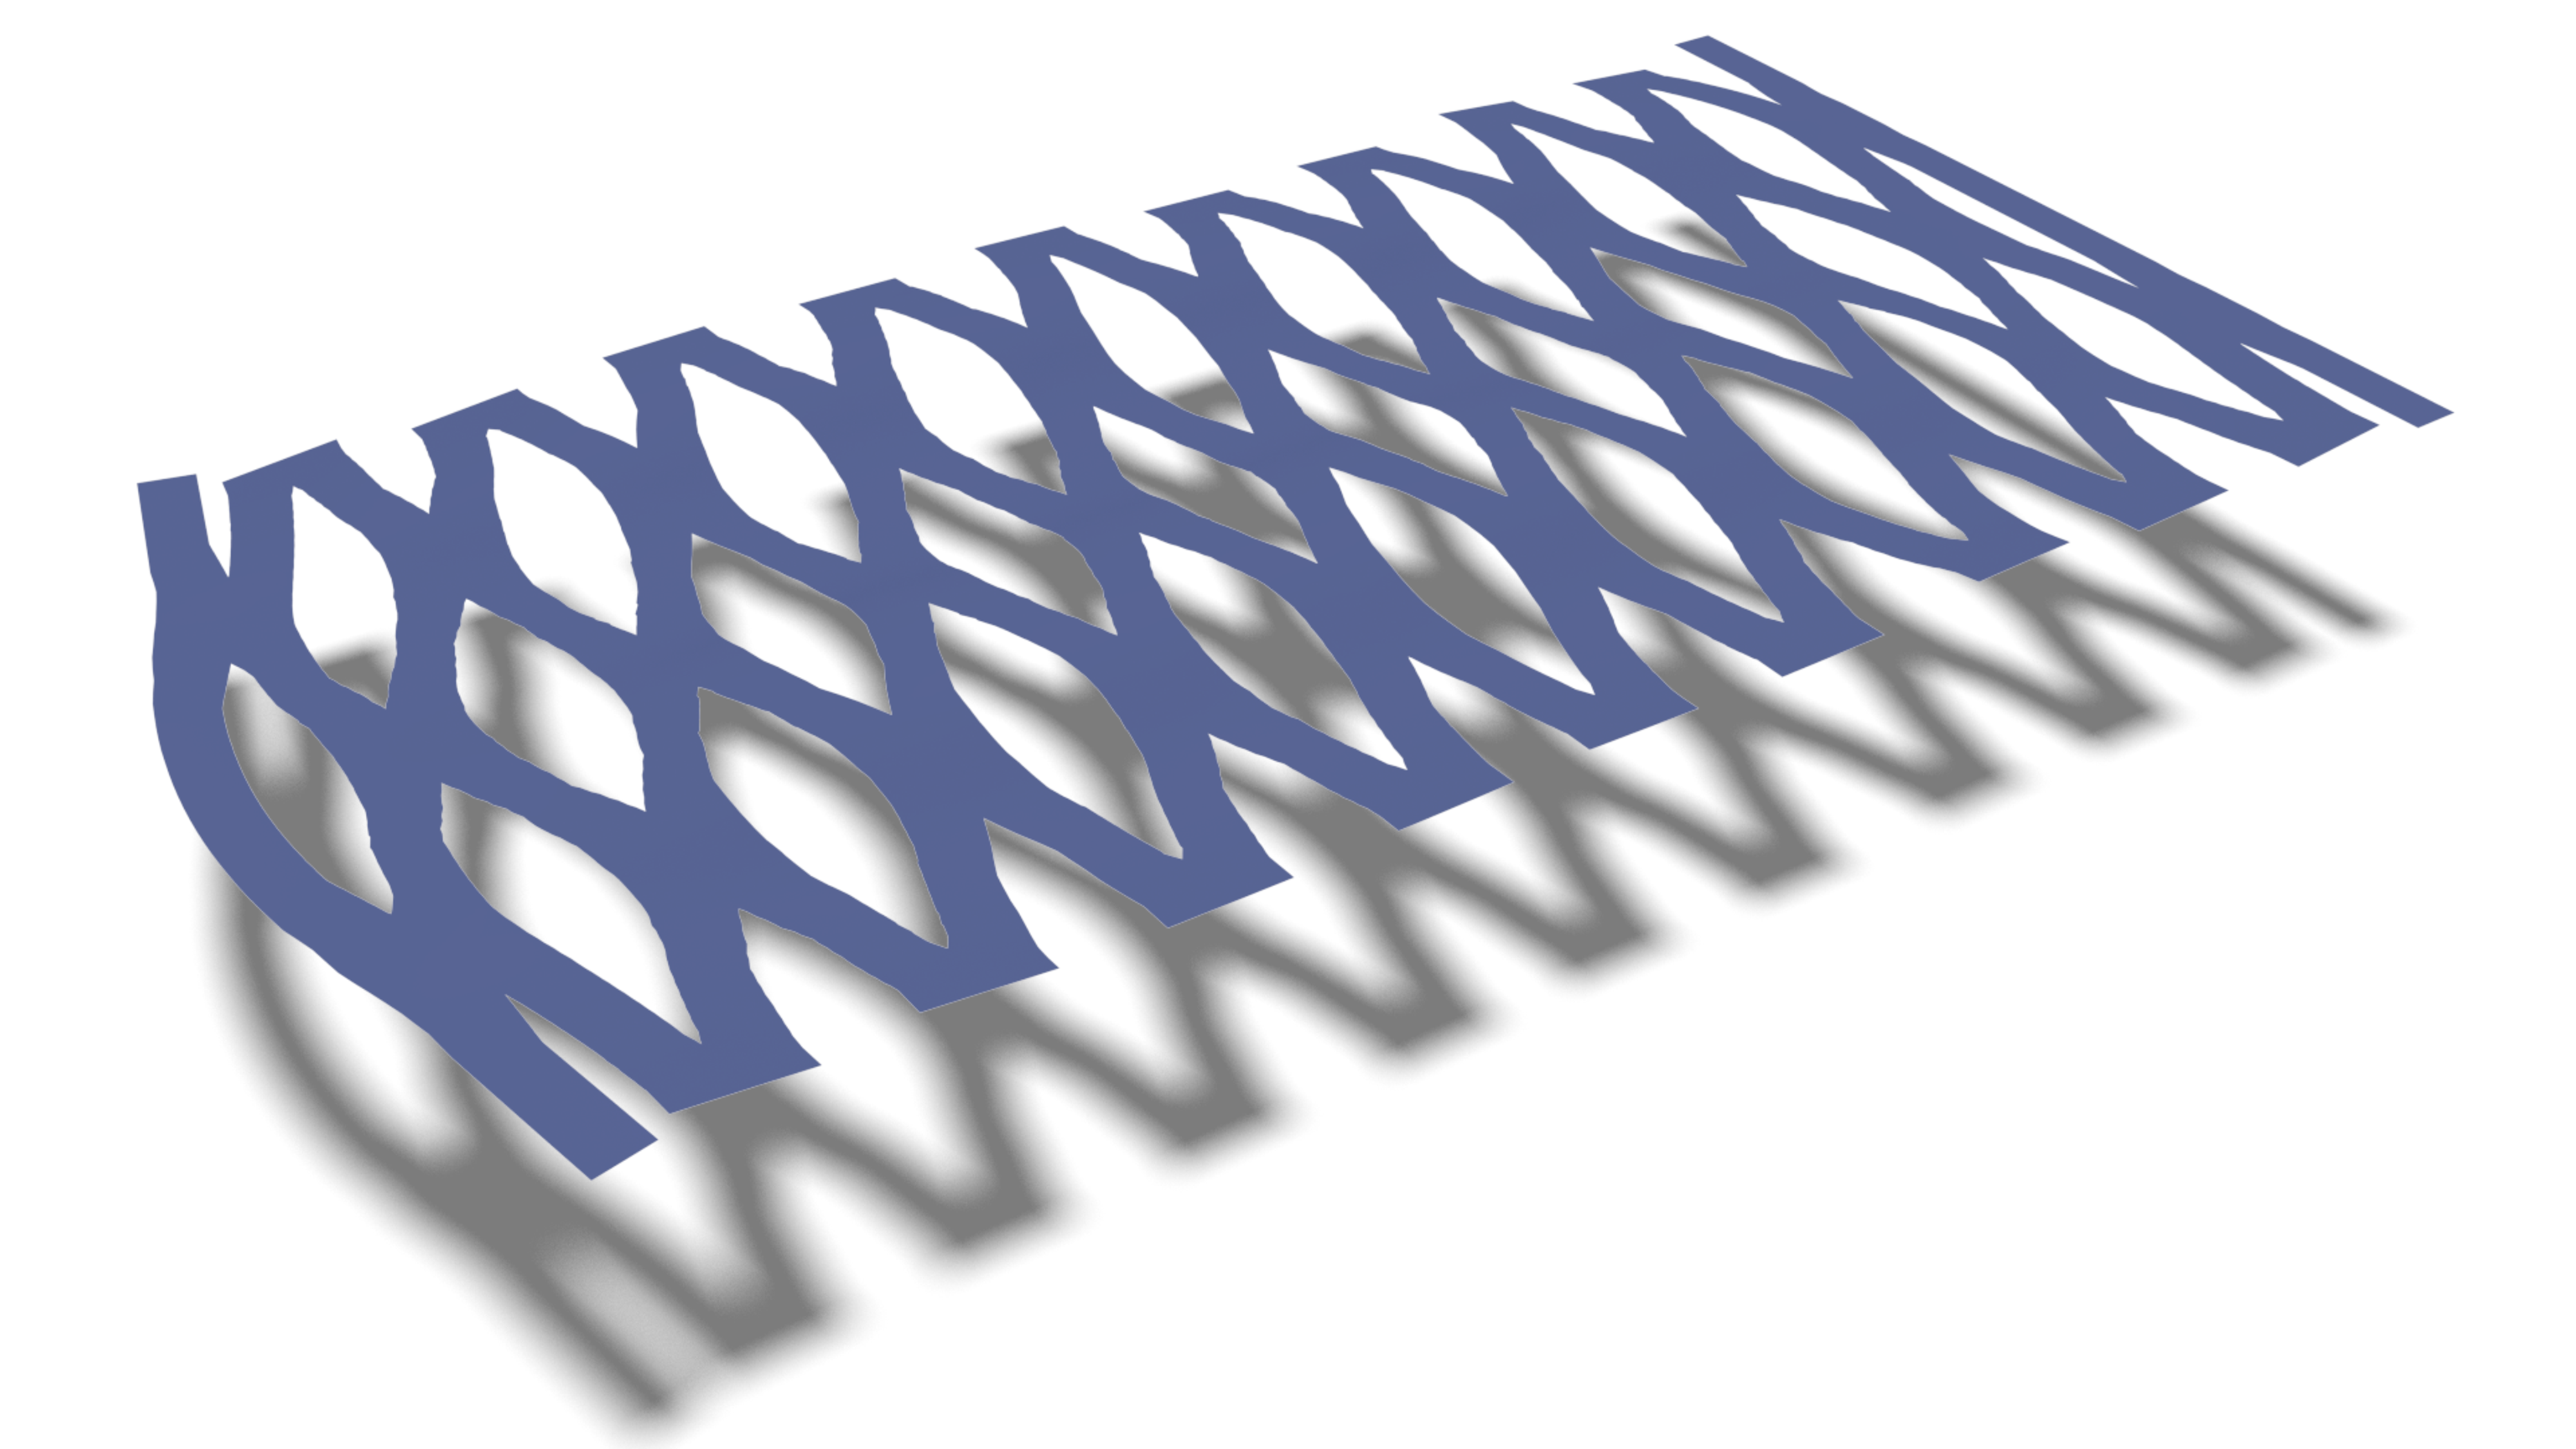
\includegraphics[width=\linewidth]{images/cutting-mig2015/Kirigami.pdf}
\caption{\label{fig:kirigami}}
\end{subfigure}
\caption{\label{fig:teaser} Progressive cutting of a spiral using only five control frames (a). Simulating complex deformations resulting from Kirigami cutting (b).}
\end{figure}

To achieve user-driven cuts in a frame-based simulation, we allow cuts to be performed on the underlying mesh.
We build a non-manifold grid that keeps track of the mesh topology at the simulation level, and allows us to incrementally adapt the frames regions of influence in order to  represent the cut.
Although remaining low, the number of frame node does increase during a cut. In particular, when a model is cut apart, at least one frame is needed to represent each disconnected component. 
Therefore, we detect crucial cutting events, enabling us to automatically insert new frames when and where they are needed.
In order to reduce computations, we exploit the locality of the ongoing cutting gesture to incrementally update all the data used for the simulation.

Our contributions include (1) the building of a non-manifold grid to compute shape functions that faithfully represent the  complex topology of the visual mesh while keeping a low number of control nodes, (2) the dynamic re-sampling of new frames into disconnected parts and (3) the incremental update of the simulation data that were concerned by the cut.

Our method can be used to simulate a wide variety of objects, such as stretchable cloth or pieces of paper. It features a very low number of frame nodes, high resolution mesh embedding, numerous and detailed cuts. Performance ranges from interactive to offline depending on the desired accuracy and complexity of the cuts.

\begin{figure*}[!ht]
\centering
\begin{subfigure}[c]{0.20\linewidth}
\centering
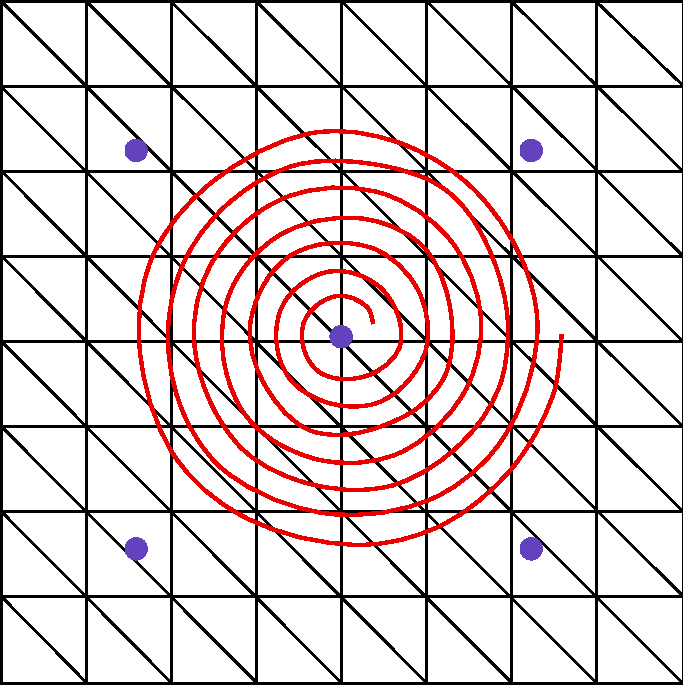
\includegraphics[width=\linewidth]{images/cutting-mig2015/spiral_mesh.pdf}
\caption{\label{fig:spiralMesh}}
\end{subfigure}
\hspace{1.5cm}
\begin{subfigure}[c]{0.70\linewidth}
\centering

\includegraphics[width=\linewidth]{images/cutting-mig2015/sfRender_ff/weightShow.pdf}
\caption{\label{fig:weightShow}}
\end{subfigure}
\caption{\label{fig:spiralWeight}
Comparison between shape functions computed on a uniform grid and on a non-manifold grid. (a) The underlying mesh (black lines) is cut by spiral (red line) and sampled with five control frames (blue circle). (b) The shape functions for each of the frame with a uniform grid (top row) and with a non-manifold grid (bottom row). Values range from $1$ to $0$ and are respectively depicted from red to blue. We can observe that shape functions computed on the non-manifold grid strictly preserve the details and topology of the underlying mesh.}
\end{figure*}
%%%%%%%%%%%%%%%%%%%%%%%%%%%%%%%%%%%%%%%%%%%%%%%%%%%%%%%%%%%%%%%%
%                       RELATED WORK
%%%%%%%%%%%%%%%%%%%%%%%%%%%%%%%%%%%%%%%%%%%%%%%%%%%%%%%%%%%%%%%%
\section{Related Work}

Cutting and fracture are both fascinating behaviors which can be simulated separately. In fracture, stress measurements predict how the material breaks. In cutting, the interaction with a tool define the cut path. For more details about cutting we refer the reader to the recent survey of Wu et al. \cite{Wu2015}. Our review focuses on the modeling of topological changes in deformable models.

A first possibility consists in using the same model for physics simulation and visualization. Topological changes are then mostly modeled by remeshing operations. Simple and fast remeshing techniques such as element deletion or element splitting were proposed. The latter was used in the first simulation of brittle and ductile materials~\cite{OBrien1999}, \cite{OBrien2002}. 
 Methods that preserve element quality by local and global remeshing have also been developed. They recently lead to stunning results in the simulation of multi-layered paper tearing~\cite{Busaryev2013} and sheets tearing \cite{Pfaff2014}. 
These methods cause the number of simulation nodes to vary over the course of a simulation, and this variation can be problematic in a realtime game context.  By limiting the
scope of remeshing predictable realtime performance can be achieved~\cite{Parker2009}.
An alternative to remeshing is to enrich elements with additional basis so that discontinuities can be represented. This is the core idea of the eXtended Finite Element Method (XFEM). It was successfully applied for offline cutting of discrete shells \cite{Kaufmann2009}.

A second possibility is to separate the visual model from the physics model, this is known as embedding. Numerous embedding techniques have been proposed. The virtual node method \cite{Molino2004} embeds ill-shaped elements that arise after remeshing inside of well-shaped elements. This allows to robustly simulate detailed cuts \cite{Wang2014}. However, the number of nodes increases substantially with the complexity of the cut. To reduce it, hierarchical methods were proposed and real-time cutting in medical applications has been achieved using composite finite element method \cite{Wu2011}. Still, the number of nodes grows quickly with the number of cuts and remains limited to ensure interactive frame rate. Meshless methods avoid the problem of element quality. However, boundary and discontinuities require extra effort to be sharply represented. \cite{Pauly2005} proposed to use visibility criterion to perform fracture. \cite{Steinemann2009} used the visual model as a visibility graph to define nodes connectivity. Both methods rely on a dense sampling near the surface of the model and quickly impact performances as the number  and the detail of cuts increases. There also have some work to carry complex materials \cite{Nesme2009} and thin shells \cite{Remillard2013} in hexahedra elements.

Embedding techniques have inspired our work. They allow interesting trade-off and show impressive cutting and fracture simulations. However, the relation between the resolution of the physical model and the visualization model remains very strong. Complex cuts result in a fast increase of the number of nodes. We want to reduce this connexion as much as possible. Complex topologies could be simulated with a very low number of nodes. Then, interactivity and intuitive control would be at hand.

Few models have been proposed that simulate detailed deformable objects using a low number of nodes. Subspace simulations \cite{Barbic2005} compute a low basis of deformation modes in order to achieve real-time performance on detailed models. However, the low-basis is acquired after heavy precomputations. Interactive scenario could not handle the recomputation of the basis at each topological change. More recently, \cite{Gilles2011} and \cite{Faure2011} proposed a physics-based skinning technique, called the frame-based method. Highly detailed meshes can be embedded in very coarse simulations. The control nodes are affine frames and the deformation field is described by a linear blend skinning. Classical continuum mechanics is then used to solve for the dynamics. Skinning weights, also called shape functions, are built on linear interpolation using discrete voronoi regions. For each frame, they can represent a large region of influence with complex shape. Other advantages are discussed in \cite{Faure2011}. Unfortunately, the current frame-based method does not allow the shape functions to reflect the topological changes of the embedded mesh.

\begin{figure*}[!ht]
\centering
\begin{subfigure}[b]{0.20\linewidth}
\centering

\includegraphics[width=\linewidth]{images/cutting-mig2015/buildSF_1.pdf}
\caption{\label{fig:buildSF1}}
\end{subfigure}
\hspace{2cm}
\begin{subfigure}[b]{0.20\linewidth}
\centering
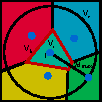
\includegraphics[width=\linewidth]{images/cutting-mig2015/buildSF_2.pdf}
\caption{\label{fig:buildSF2}}
\end{subfigure}
\hspace{2cm}
\begin{subfigure}[b]{0.20\linewidth}
\centering
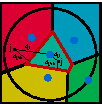
\includegraphics[width=\linewidth]{images/cutting-mig2015/buildSF_3.pdf}
\caption{\label{fig:buildSF3}}
\end{subfigure}
\caption{\label{fig:shapefunctionconstruction}
Illustrations of Voronoi shape function computation. (a) Starting from samples (blue circles), we build a Voronoi diagram using Dijkstra's shortest path algorithm. (b) Then, for each frame and its region $V_{i}$, we compute the maximum distance $d_{max}$ to its Voronoi boundary $V_{b}$. We extend $V_{i}$ to twice $d_{max}$ which gives $V_{e}$. (c) Finally for each grid cell $j$ in $V_{e}$ we linearly interpolate using distance to the frame position and distance to $V_{b}$.}
\end{figure*}

\section{Overview}

The goal of this work is to enable interactive detailed cutting of deformable thin sheets. The frame-based method exhibits some of the key features we are looking for: a very low number of nodes and a tunable separation between visual and physical models.  We build on this framework and extend it to handle topological changes.

To transfer the cuts from the mesh to the frames, we continuously adapt the shape functions to the evolving mesh topology. This allows us to keep a constant number of nodes as long as there are no disconnected parts. In \cite{Faure2011}, the shape functions are computed on a uniform grid. The structure is simple and efficient. However, discontinuities that can be represented are very limited and strongly connected to the grid resolution. Instead, we build a non-manifold grid to compute topology-preserving shape functions (see Figure \ref{fig:spiralWeight}). The main idea is that cut cells are duplicated and store different connectivities. Therefore, grid resolution depends much less on the mesh topology while keeping all topological informations.

We detail the computation of the shape functions, motivate the use of a non-manifold grid and explain how to build it (Section \ref{sec:adaptivesf}). When several parts are disconnected, we need to make sure that they contain control frames. We present a simple method to detect those regions and re-sample them (Section \ref{sec:resampling}). Even with such a low resolution physics model, it would be overkilling to update the whole system at each cut. Fortunately, cutting is often a local event. We leverage this fact and propose simple strategies to incrementally update the different components of the simulation (Section \ref{sec:incremental}). We illustrate our method in different scenarios (Section \ref{sec:results}) and discuss limitations and future work (Section \ref{sec:discussion}). We summarize our simulation loop in Algorithm~\ref{alg:simulationLoop} and detail our remeshing algorithm in appendix~\ref{appendix:remeshing}.

\begin{algorithm}[h]
\caption{\label{alg:simulationLoop}Simulation loop}
\begin{algorithmic}[0]
\For{each time step}
	\State perform a frame-based simulation step
	\State split the mesh along the cut
	\State embed the mesh in a non-manifold grid
	\State add new frames if required
	\State add new samples (collision, integration) if required
	\State compute shape functions on the grid
	\State incrementally update the samples
\EndFor
\end{algorithmic}
\end{algorithm}

\begin{figure*}[!ht]
\centering
\begin{subfigure}[b]{0.20\linewidth}
\centering
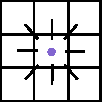
\includegraphics[width=\linewidth]{images/cutting-mig2015/connectivity.pdf}
\caption{\label{fig:connectivity}}
\end{subfigure}
\hfill
\begin{subfigure}[b]{0.30\linewidth}
\centering
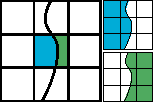
\includegraphics[width=\linewidth]{images/cutting-mig2015/simple_cut.pdf}
\caption{\label{fig:simplecut}}
\end{subfigure}
\hfill
\begin{subfigure}[b]{0.40\linewidth}
\centering
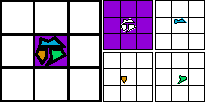
\includegraphics[width=\linewidth]{images/cutting-mig2015/little_pieces.pdf}
\caption{\label{fig:littlePieces}}
\end{subfigure}
%\hfill
%\begin{subfigure}[b]{0.24\linewidth}
%\centering
%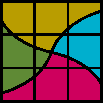
\includegraphics[width=\linewidth]{images/cutting-mig2015/multi_cut.pdf}
%\caption{\label{fig:multicut}}
%\end{subfigure}
\caption{\label{fig:nonmanifoldgridillustration}
Illustrations of different possibilities for a non-manifold cell with eight connectivity (a). In (b), the cell is simply cut into two cells. Each duplicate of the cut cell has a specific connectivity that represent the cut topology. In (c), multiple disconnected components can be contained inside one cell. The cell is duplicated four times. Three of the duplicates have no connectivity. However they can embed complex geometry and then be simulated by adding new frames for each of the component. The fourth duplicate keeps its eight neighbors and remains independent from the three other.}
\end{figure*}

%%%%%%%%%%%%%%%%%%%%%%%%%%%%%%%%%%%%%%%%%%%%%%%%%%%%%%%%%%%%%%%%
%                      WEIGHT COMPUTATION / GRID
%%%%%%%%%%%%%%%%%%%%%%%%%%%%%%%%%%%%%%%%%%%%%%%%%%%%%%%%%%%%%%%%
\section{Adaptive shape functions} \label{sec:adaptivesf}

In this section, we first summarize how Voronoi shape functions are traditionally computed. Then we detail why a non-manifold grid is necessary, how to build it and how to use it to compute the shape functions on complex topology.

%%%%%%%%%%%%%%%%%%%%%%%%%%%%%%%%%%%%%%%%%%%%%%%%%%%%%%%%%%%%%%%%
%                      SHAPEFUNCTION
%%%%%%%%%%%%%%%%%%%%%%%%%%%%%%%%%%%%%%%%%%%%%%%%%%%%%%%%%%%%%%%%
\subsection{Voronoi shape function}

Let $w_{i}(x) : \Omega \rightarrow \mathcal{R}$ be the shape function for the $i$-th control frame, where $\Omega$ represents the domain. Starting from the Voronoi partition $V$ of the set of control frames, we can independently compute $w_{i}$ for each frame.

First, we compute the maximal distance $d_{max}$ from the control node to its Voronoi boundary $V_{b}$. Then we extend its Voronoi region $V_{i}$ to twice $d_{max}$. This gives a new region $V_{e}$ which describes the final boundary of the shape function. Now, we can compute $w_{i}$ inside $V_{e}$. We set $w_{i}$ to be $1$ at the frame position, $0$ at the others and $0.5$ on $V_{b}$. Finally, we linearly interpolate $w_{i}$ between $V_{b}$, the frame position and the boundary of $V_{e}$. We detail the interpolation in Algorithm~ \ref{alg:shapefunctioncomputation} and in Figure~ \ref{fig:shapefunctionconstruction}.

In practice, Voronoi diagram is computed using Dijkstra's shortest path algorithm on a grid in order to preserve geodesic distances. For each frame, the shape function is computed on the whole grid. As the grid resolution can be quite coarse, this is particularly fast. Negative values are clamped and weights are normalized to form a partition of unity. Then least-square approximation is performed to evaluate the shape function and its derivatives at specific position.

\begin{algorithm}[h]
\caption{\label{alg:shapefunctioncomputation}Shapefunction computation}
\begin{algorithmic}[1]
\Procedure{Compute$\_$Shapefunction}{}
\For{each frame $i$}
	\State $V_{i} \gets$ Voronoi region of $i$
	\State $V_{b} \gets$ boundary of $V_{i}$	
	\State $d_{max} \gets$ maximum distance to $V_{i}$ boundary
	\State $V_{e} \gets$ extend $V_{i}$ to $2.0 \times d_{max}$
	\LineComment{dist($A$,$B$) is the geodesic distance between $A$ and $B$}
	\For{each grid cell $j$ in $V_{e}$}
	\If{$j$ is inside $V_{i}$}
	\State $\displaystyle w_{i}(j) = 0.5\left(1 + \frac{dist(j,V_{b})}{dist(j,V_{b})+dist(j,i)}\right)$
	\ElsIf{$j$ is inside $V_{e}$}
		\State $\displaystyle w_{i}(j) = 0.5\left(1 - \frac{dist(j,V_{b})}{dist(j,i)-dist(j,V_{b})}\right)$
	\EndIf
	\EndFor
\EndFor
\EndProcedure
\end{algorithmic}
\end{algorithm}

Voronoi shape functions were designed in order to respect key properties that are particularly useful for physics-based animation \cite{Faure2011} . First, they respect the Kronecker property, i.e $w_{i}(x) = \delta_{i}(x)$ where $w_{i}(x)$ is the shape function of node $i$, $x$ is a spatial position and $\delta_{i}$ is Dirac function. Second, they form a partition of unity, i.e $\sum_{i}w_{i}(x) = 1$. Third, they are built to be as linear as possible in order to produce uniform deformations. Finally, they can easily be biased by material properties in order to represent heterogeneous material.

%In the extension of the frame-based method \cite{Faure2011}, they propose to use Voronoi shape functions. In this method, the region of influence of each frame is defined by an extension of its voronoi region. Weights are linearly interpolated between the position of the frame and the boundary of the initial voronoi region and they are extrapolated between the boundary of the initial voronoi and the boundary of the extended voronoi. In their paper, the voronoi diagrams are computed on a discrete grid with a 8 neighbor connectivity using a Dijkstra algorithm. Weights and weight derivatives are then interpolated to specific sample positions such as mesh vertices or integration points or collision points. Weights are ensured to be linear along shortest path. This method allows to biase the distance computation by a material map in order to build weights that can represent heterogenous material. In our method we use the same shape functions in order to represent large regions and hetergenous materials. However we need to adapt the shape functions along the simulation to take into accounts the cuts.
%Shape functions describe the influence region of each node. In linear finite element methods, this region is clearly delimited by the elements that surrounds each vertex. Thus topology is naturally represented by the mesh itself. In mesh-less methods, 
%Each vertex influence 
%barycentric linear shape functions are used in triangular and tetrahedral meshes. They naturally represent the topology of the mesh and produce uniform deformations. In mesh-less methods, each node 
%The design of shape functions for skinning deformation is an active topic of research. Several key features have been identified in order to produce plausible deformations.
%Three key features that ensure plausible deformations have been identified. The first one is that the shape function should decrease with respect to the distance from the corresponding control node. The second one is that it should be as linear as possible in order to produce uniform deformations. Finally, it should respect the Kronecker property in order to provide easy  manipulations.
%Usually, three key features should be preser
%They should  Generally, the function decreases from $1$ to $0$ from the node position 
%Linear shape functions ensure that the material deform uniformly with the frame motions. 
%Usually, we want the region attached to a node to deform uniformly with it. Therefore we use linear weights
%the region of influence of each control frame
%The design of skinning weights is an active topic of research.
%Skinning weights describe the region of influence of the control frames and the type of influence. Generally we want the space to deform uniformly with the frames and so we use linear weights. When the region of a node is a simple shape such as a set of triangles or a quads, one can use well known weights such as barycentric or bilinear weights. However, when we do not want to describe the deformation field using a specific geometry, it is much more challenging to design shape functions. Most of the meshless methods use overlapping spline kernel with local support to describe the deformation field. Unfortunately this requires relatively dense sampling to cover the whole region. Nevertheless, both methods use local shape functions and assume that the number of nodes is important. In procedural animation, design of skinning weights is an active topic of research. The goal is to design weight that can cover regions of different sizes, while respecting the topology in order to provide intuitive control of a shape. An important step was achieved by the work of \cite{Joshi2007} where they propose to use harmonic coordinates. Those skinning weights provide control over large regions while keeping the coherency of the topology. Unfortunately, those weights are highly nonlinear and results in unconvining behavior in physics-based simulation. 

\subsection{Non-manifold grid}

As mentionned above, in \cite{Faure2011}, shape functions are computed on a uniform grid using Dijktra's shortest path algorithm to compute geodesic distance. Starting from a uniform grid with a 8-neighbor connectivity, we could reflect topological change by changing the connectivity of the cut cells. Then, when we re-compute shape functions, the topology would automatically be taken into account as we use geodesic distance. 

Unfortunately, this strategy is very limited for uniform grid and would only work in simple cases. For instance, several cuts that intersect or that create disconnected components inside one cell could not be represented. Even without cut, small gaps that lie inside one cell could not be correctly represented. Geodesic distances would be false and the object would behave as if there were no cuts or gaps. Augmenting the resolution would not solve the problem. We would fight the same issue as previous methods. Our grid resolution would be highly dependent on the complexity of the topology and the geometry of the object. It would directly impact performances.

We want each grid cell to be able to represent  the connectivities of the different disconnected components that lie in the cell. To do so, each cut cell is duplicated as many times as it contains disconnected parts. Each duplicate has a specific connectivity built from the material connectivity. This results in a data structure called \emph{non-manifold grid} (see Figure \ref{fig:nonmanifoldgridillustration}).

Non-manifold grids are used by many other cutting methods to embed fine geometric details in coarse finite element simulations. However, we make a completely different use of it. Instead of duplicating control nodes as the cells are cut, thereby increasing their number and the computation time, we use the grid to adapt the shape functions to the evolving topology of the mesh. Most of the time, the number of nodes can remain constant while representing detailed geometry and multiple cuts.

There are several ways to compute this non-manifold grid. In our method, we start by embedding the mesh in a uniform grid. Mesh elements that overlap a grid cell are detected using intersections tests and are assigned to it. Then, for each grid cell, we use a flood fill algorithm to detect the disconnected parts of the mesh. This informs about how many duplicates need to be created for the cell. Finally, for each duplicate we establish its connectivity by comparing its geometry with the geometry of the neighbor cells duplicates. We summarize our method in Algorithm~\ref{alg:nonmanifoldbuilding} and illustrate the main steps in Figure~\ref{fig:nonmanifoldgridbuilding}.

\begin{algorithm}[!ht]
\caption{\label{alg:nonmanifoldbuilding}Non-manifold grid building}
\begin{algorithmic}[1]
\Procedure{Build$\_$Non$\_$Manifold$\_$Grid}{grid $G$, mesh $M$}
\State \textsc{Build$\_$Grid$\_$Geometry}($G$,$M$)
\State \textsc{Duplicate$\_$Grid$\_$Cell}($G$)
\State \textsc{Build$\_$Grid$\_$Connectivity}($G$)
\EndProcedure
\State
\Procedure{Build$\_$Grid$\_$Geometry}{grid $G$, mesh $M$}
\For{each cell $i$ of $G$}
\State Store overlapping element of $M$
\EndFor
\EndProcedure
\State
\Procedure{Duplicate$\_$Grid$\_$Cell}{grid $G$, mesh $M$}
\For{each cell $i$ of $G$}
\State $C \gets $ disconnected component of $M$ in $i$
\For{each component j of $C$}
	\State Duplicate the cell $i$
	\State Store $j$ in the duplicate
\EndFor
\EndFor
\EndProcedure
\State
\Procedure{Build$\_$Grid$\_$Connectivity}{grid $G$}
\For{each cell $i$ of $G$}
\State $N \gets $ neighbor cells of $i$
\For{each duplicate $j$ of $i$}
\For{each duplicate $k$ in $N$}
\If{$j$ and $k$ shares geometry}
\State Create a link between $j$ and $k$ 
\EndIf
\EndFor
\EndFor
\EndFor
\EndProcedure
\end{algorithmic}
\end{algorithm}

\begin{figure*}[!ht]
\centering
\begin{subfigure}[b]{0.20\linewidth}
\centering
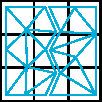
\includegraphics[width=\linewidth]{images/cutting-mig2015/buildNMG_1.pdf}
\caption{\label{fig:buildNMG1}}
\end{subfigure}
\hfill
\begin{subfigure}[b]{0.20\linewidth}
\centering
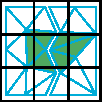
\includegraphics[width=\linewidth]{images/cutting-mig2015/buildNMG_2.pdf}
\caption{\label{fig:buildNMG2}}
\end{subfigure}
\hfill
\begin{subfigure}[b]{0.20\linewidth}
\centering
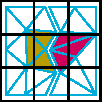
\includegraphics[width=\linewidth]{images/cutting-mig2015/buildNMG_3.pdf}
\caption{\label{fig:buildNMG3}}
\end{subfigure}
\hfill
\begin{subfigure}[b]{0.20\linewidth}
\centering
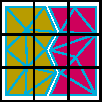
\includegraphics[width=\linewidth]{images/cutting-mig2015/buildNMG_4.pdf}
\caption{\label{fig:buildNMG4}}
\end{subfigure}
\caption{\label{fig:nonmanifoldgridbuilding}
We describe the building of the non-manifold grid for the center cell of the grid. (a) The mesh is embedded in a uniform grid. (b) First, we store the overlapping geometry in the cell. (c) Then we detect disconnected parts using a flood fill algorithm. (d) Finally the cell is duplicated. For each duplicate, we look for other duplicates that share geometry and establish its connectivity.}
\end{figure*}

%%%%%%%%%%%%%%%%%%%%%%%%%%%%%%%%%%%%%%%%%%%%%%%%%%%%%%%%%%%%%%%%
%                      FRAME RESAMPLING
%%%%%%%%%%%%%%%%%%%%%%%%%%%%%%%%%%%%%%%%%%%%%%%%%%%%%%%%%%%%%%%%

\section{Frame re-sampling} \label{sec:resampling}
As long as no parts of the model are disconnected, our method allows to keep a constant number of control frames. However, when parts are disconnected, we need to sample it with at least one frame in order to simulate it. 

We start by detecting empty regions i.e lists of connected cells that are not influenced by any frame. This is done using a flood fill algorithm on the grid containing the shape functions values. These empty regions are then sampled using a farthest sampling algorithm. Finally, the samples are uniformly distributed by applying several Lloyd relaxation steps. For now, the number of frames which are sampled is user-defined but we would like to investigate for setting it automatically (see Section \ref{sec:discussion}). 

As a cut progresses, it may happen that only one frame influences a large region. Then this region can only express affine motion. Depending on the material properties, the size and the shape of the region, this can result in unconvincing behaviours. For rigid materials this is not a problem but for soft material this can quickly become unrealistic. We propose a simple strategy to solve some of these cases. For each frame, we look for regions where the shape function value is above a user-defined threshold $w_{max}$. Then if the volume of the region is above a maximal volume threshold $v_{max}$, we uniformly re-sample the region. This strategy allows to detect large regions which are mostly influenced by only one frame and are the most likely to need re-sampling. For now, $w_{max}$ and $v_{max}$ are user-defined.

As regions of influence are very large, the popping artefacts induced by adding instantaneously one additional frame can be noticeable. In order to reduce them we propose a simple strategy. Once the position of the new frame in the undeformed, material space has been chosen, we use the previous deformation field to interpolate its new position, orientation and velocity.

%%%%%%%%%%%%%%%%%%%%%%%%%%%%%%%%%%%%%%%%%%%%%%%%%%%%%%%%%%%%%%%%
%                      INCREMENTAL UPDATE
%%%%%%%%%%%%%%%%%%%%%%%%%%%%%%%%%%%%%%%%%%%%%%%%%%%%%%%%%%%%%%%%
\section{Incremental update} \label{sec:incremental}

The domain and the shape functions continuously change during cutting. Therefore, all the simulation data that are related to the domain or the shape functions need to be updated at each time step a cut occurs. Fortunately, cutting is often a local phenomenon. We exploit this locality to incrementally update only what is necessary and therefore save substantial computational time.

In our case, there are several simulation components that need to be updated. The first of this component contains the integration points that compute deformation gradients and transfers internal forces to the control frames. Then there is the collision component, a simple set of points, that transfers external forces to the control frames. Finally, there is the mesh that we visualize whose vertices positions are interpolated from the frame positions. Each of this component can have its own resolution. Their data are computed from the control frames using interpolation. This layer-based organization allows to separate the resolutions of the physical simulation, the interactive model and the visual rendering to achieve a good trade-off between realism and performance.

In the following sections we describe the mechanisms we used to incrementally update the different components of the simulation.

\subsection{Re-sampling}
\label{sec:all_resampling}
As for the frames, we always need to have at least one collision node and one integration point inside each part of the model. Otherwise, we cannot compute deformations or interact with these parts of the model. Usually, there are much more collision nodes and integration points than frames. Instead of adding new points only when we detect new empty regions, we perform a few Lloyd relaxation steps at each time step to always keep a uniform sampling of the domain. In a progressive cut scenario, only a small number of samples will need to be updated at each time step and will result in an efficient incremental update. However, if disconnected parts are created from a cut, we apply the re-sampling strategy discussed in Section \ref{sec:resampling}. We detect the disconnected parts using a flood fill algorithm and uniformly re-sample them.

\subsection{Integration point update}
\label{sec:gausspointupdate}

Integrations points are used to compute deformation gradients and transfer internal forces to the frames. To do so, each integration point are interpreted as a small volume of the domain and carries a position, a region's volume and the volume moments. As soon as a cut occurs, the region's volume of integration points close to the cut will change and it becomes necessary to update these integration points. This can be easily done by storing an explicit description of the region of the integration point i.e a list of cells. If the cut goes through one of these cells then we update the integration point data.

\subsection{Local weights update} \label{sec:interpolation}

Weights and derivatives are interpolated from the grid to positions of the different samples : collision nodes, integration points and mesh vertices. At each cut, we need to update these values. In an interactive context, we cannot afford to perform interpolation for all these samples. Once again, we leverage the fact that a cut is very often a local event, sometimes progressive, and will impact only a small fraction of the different samples. Our idea is to perform incremental update of weights and derivatives by detecting the low number of samples that were impacted by the cut. At each time step, if a cut was performed, we compare the new shape functions with the previous ones and detect the grid cells which have been impacted by the cut. All the samples that are contained or are neighbors of these cells need to be updated. In the end, even if we have control frames that covers large regions of the domain compared to classical simulations, simulation data that need to be updated remains spatially local.
\begin{figure*}[ht]
\centering
\begin{subfigure}[c]{0.33\linewidth}
\centering
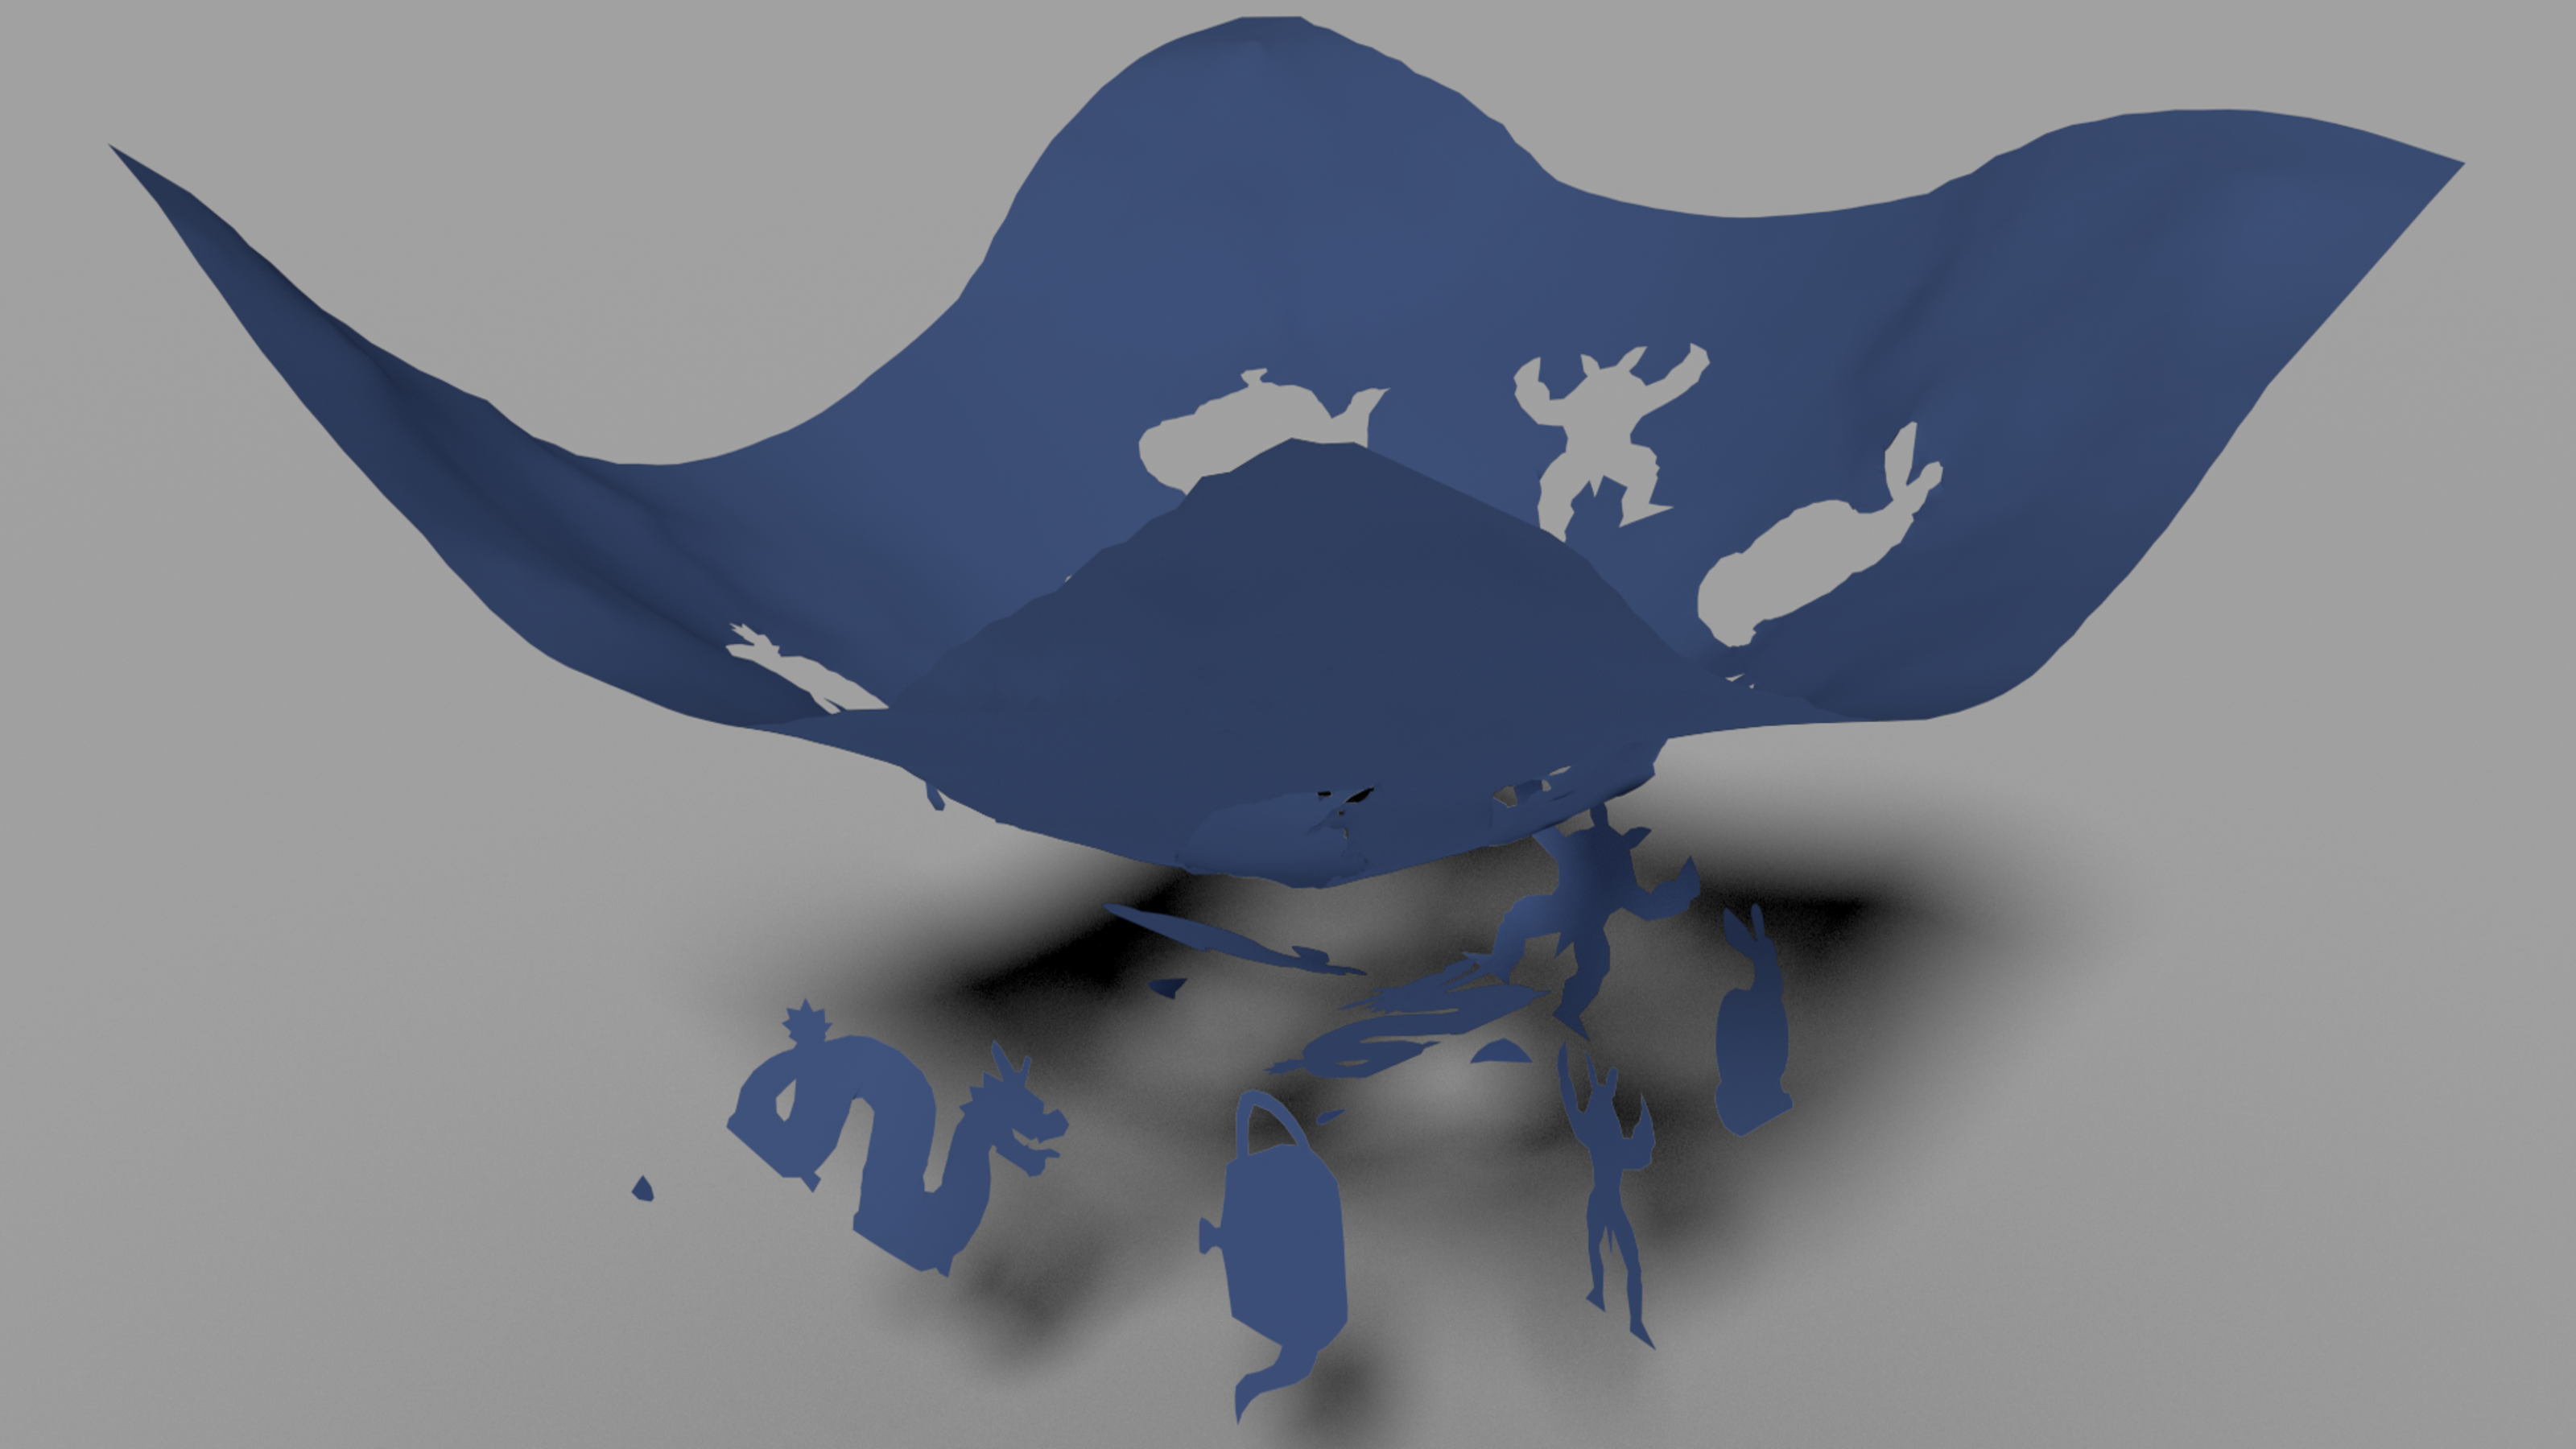
\includegraphics[width=\linewidth]{images/cutting-mig2015/Patchwork.pdf}
\caption{\label{fig:patchwork}}
\end{subfigure}
\hfill
\begin{subfigure}[c]{0.33\linewidth}
\centering
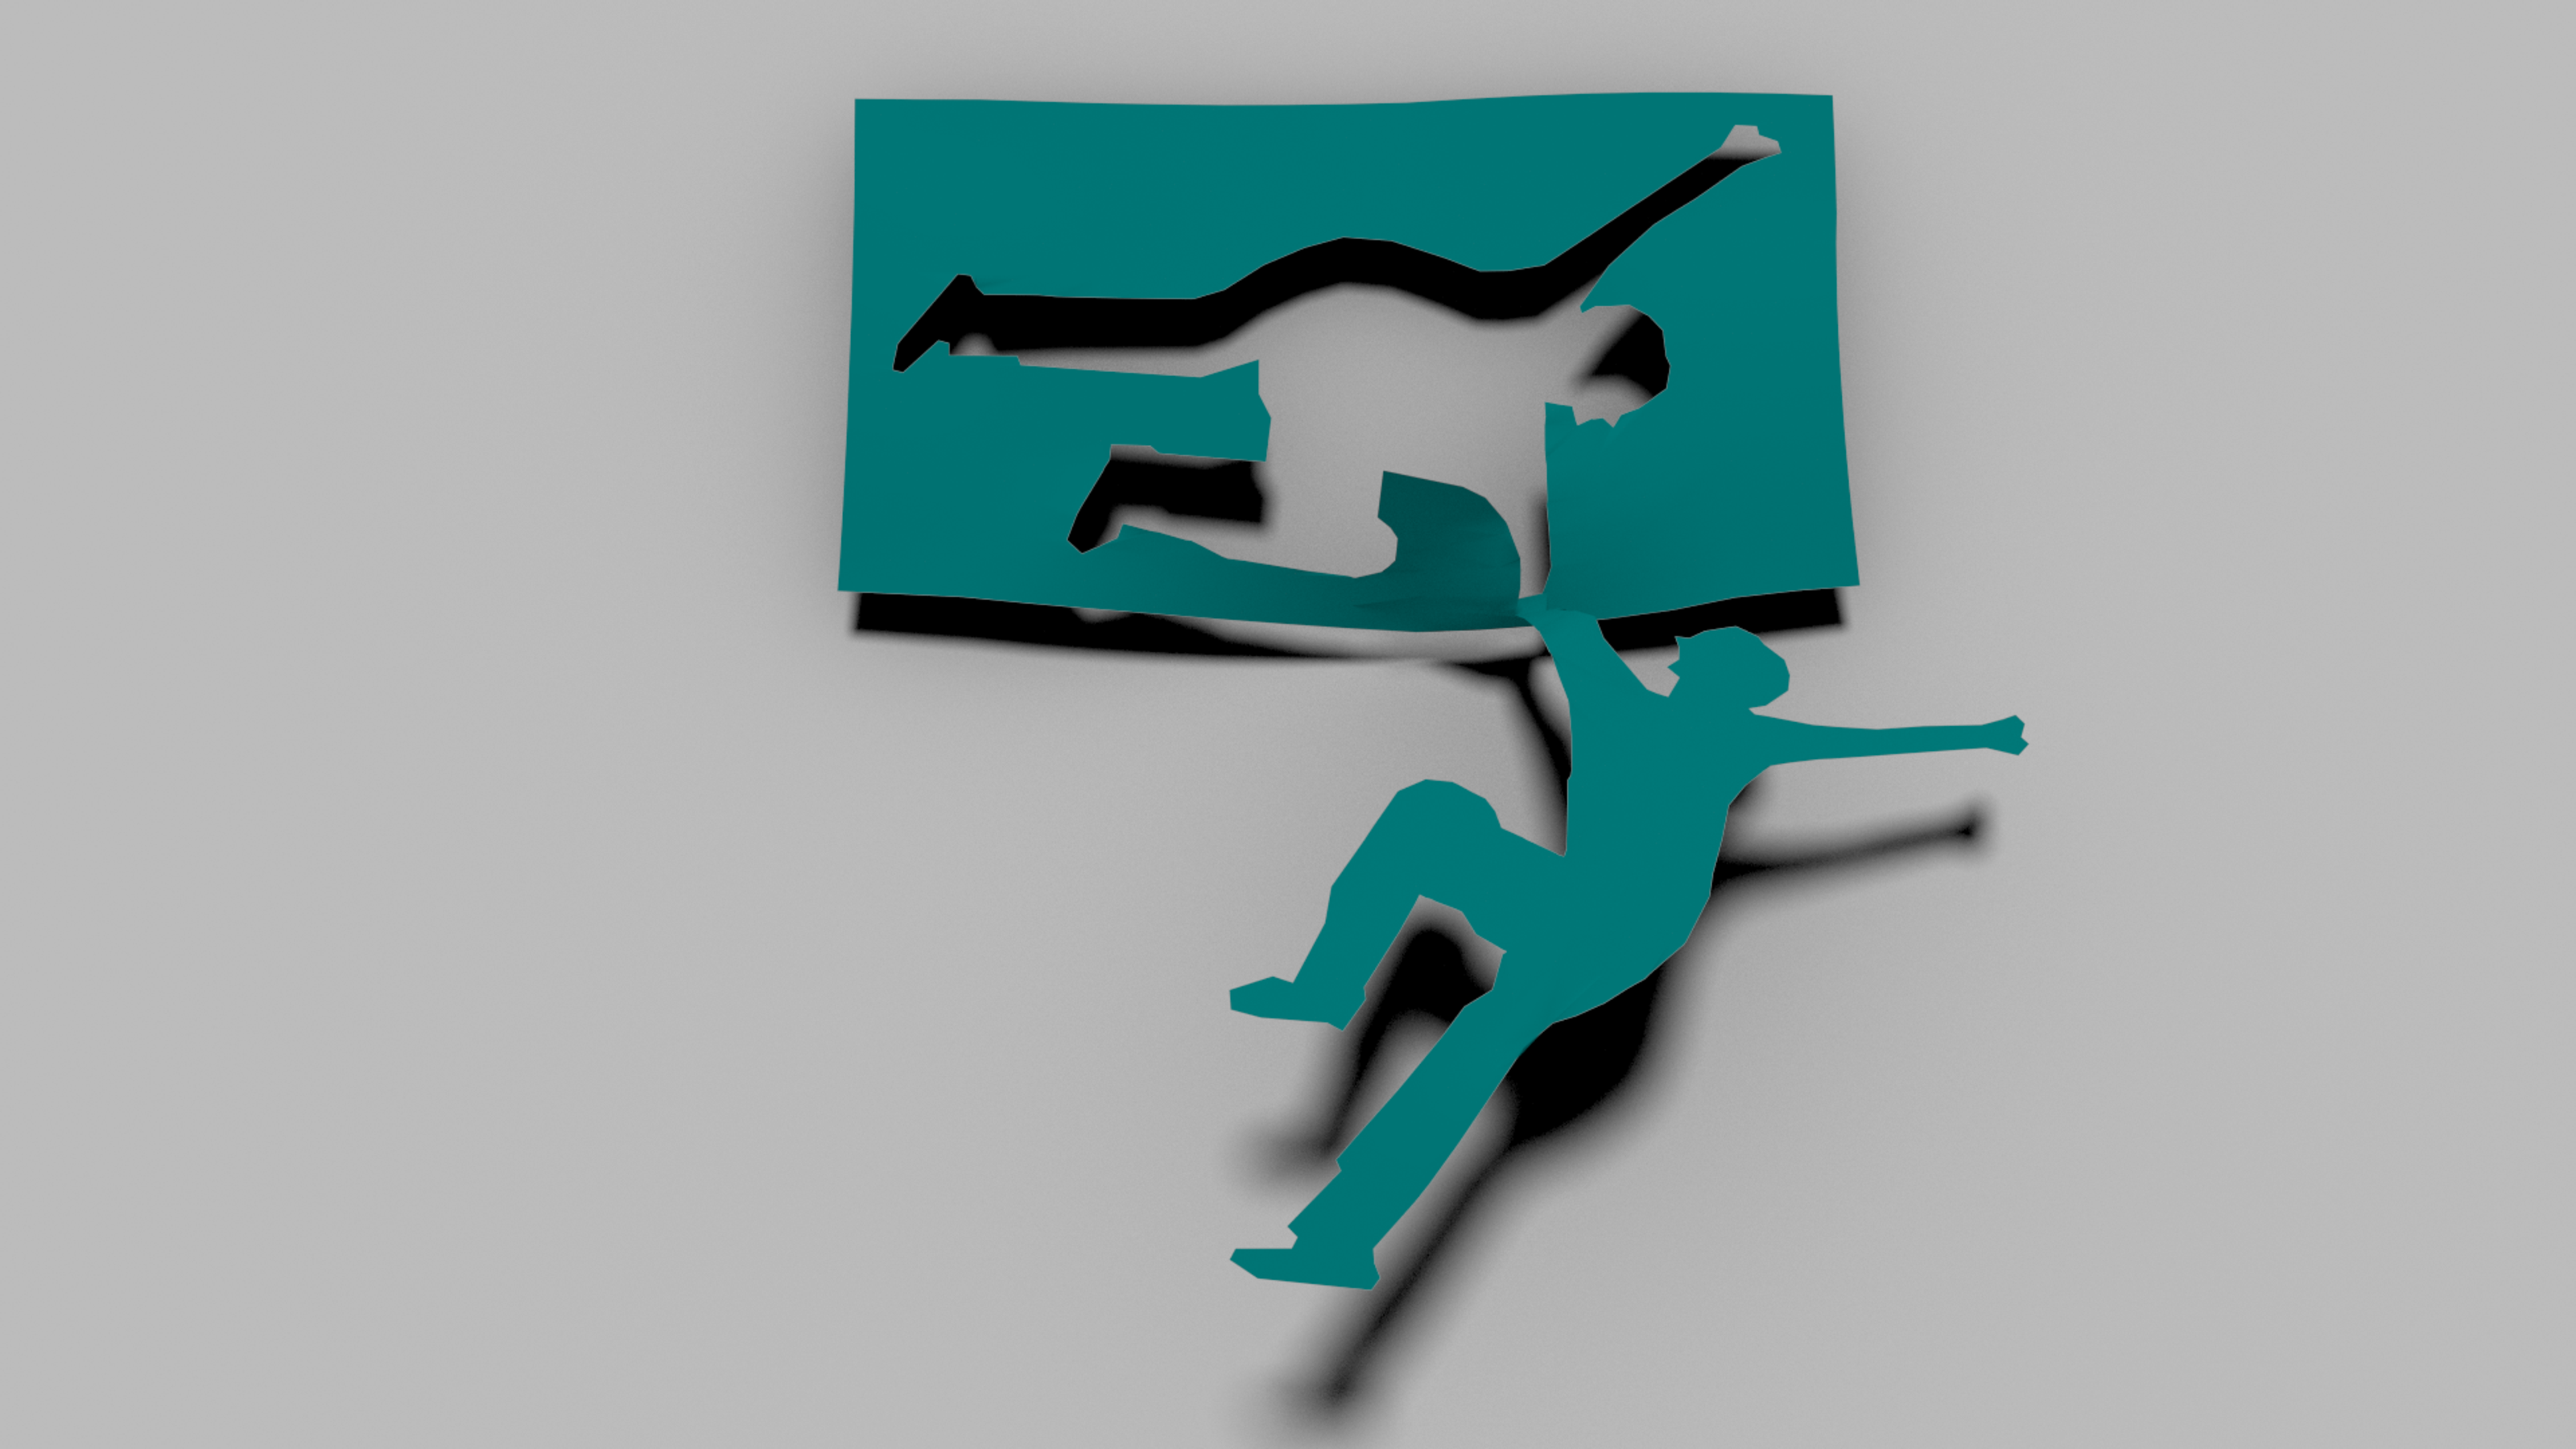
\includegraphics[width=\linewidth]{images/cutting-mig2015/FallingGuy.pdf}
\caption{\label{fig:fallingguy}}
\end{subfigure}
\hfill
\begin{subfigure}[c]{0.33\linewidth}
\centering
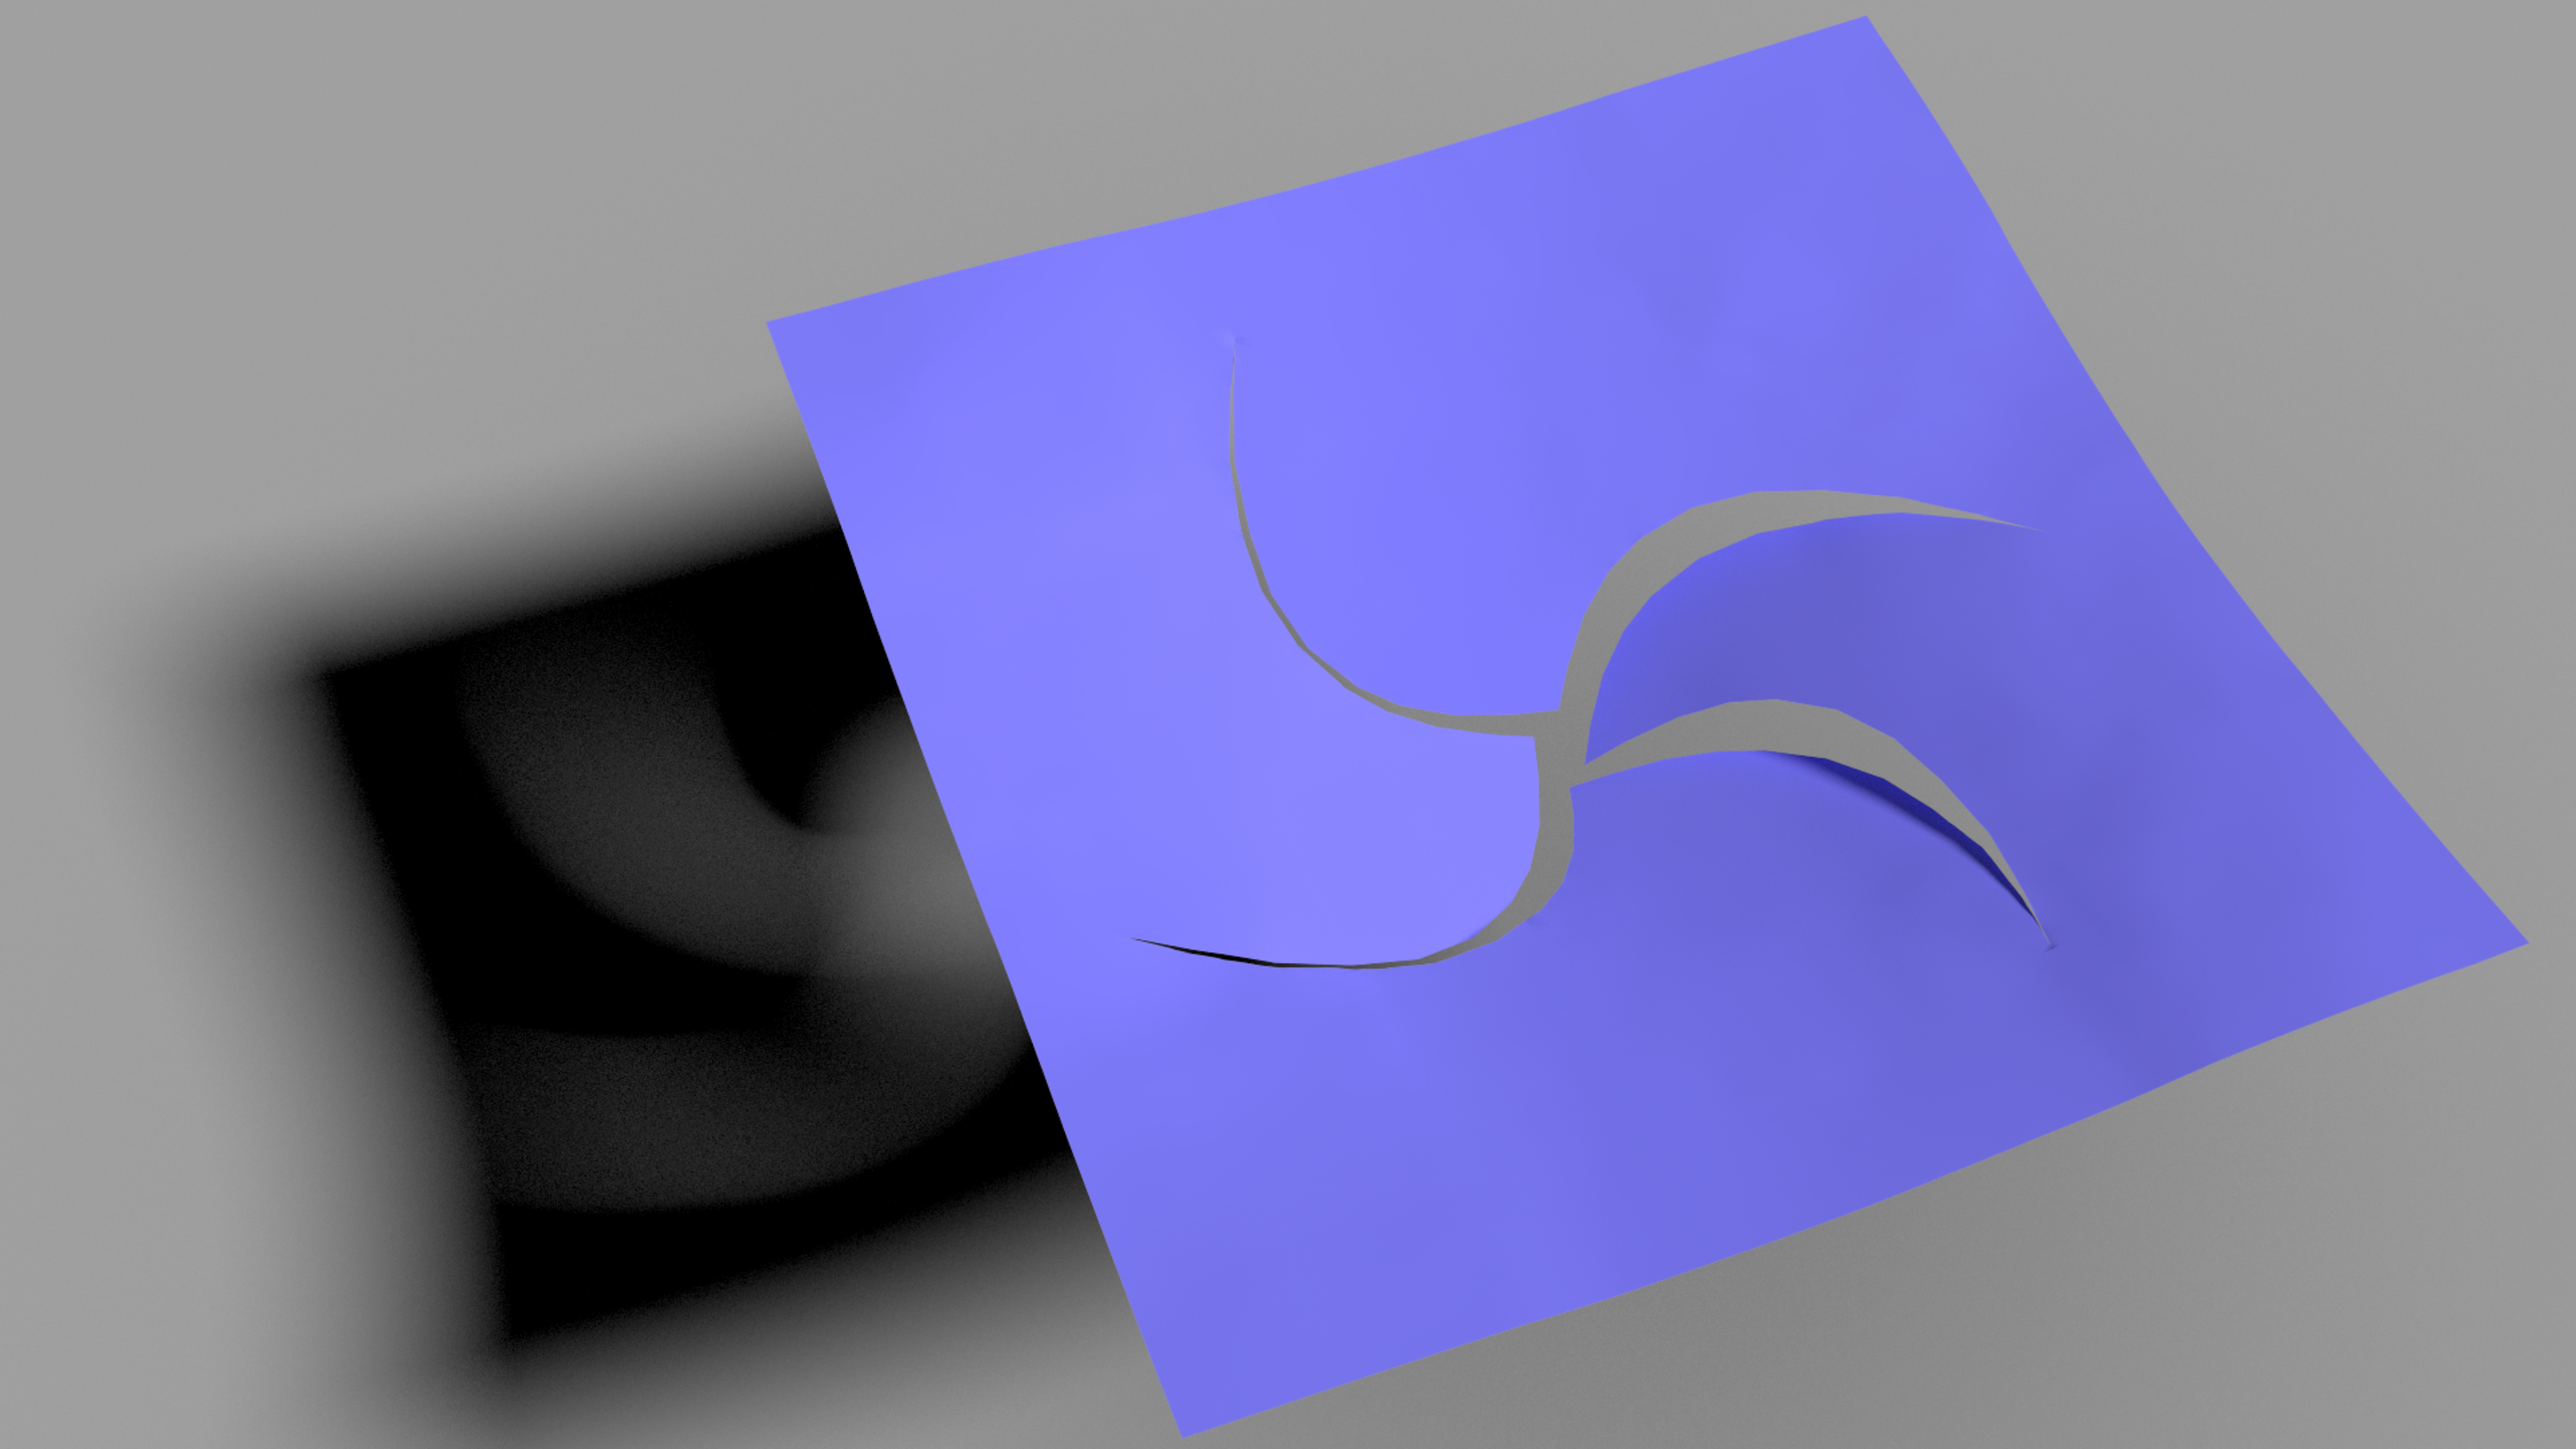
\includegraphics[width=\linewidth]{images/cutting-mig2015/Vortex.pdf}
\caption{\label{fig:vortex}}
\end{subfigure}
\caption{\label{fig:result} (a) Several highly detailed shapes are cut in a deformable sheet. Each disconnected part is automatically re-sampled with additional control frames. (b) Simulation of a highly detailed cut that falls under gravity and remains attached to the main part by a thin piece of paper. (c) Two cuts intersect to form a vortex shape. This illustrates the abilities of the non-manifold grid to handle multiple intersecting cuts.}
\end{figure*}

\addtolength{\tabcolsep}{-1.5pt}
\begin{table*}[!ht]
\centering
\begin{tabular}{l|c|cc|cc|c|c|ccc}
& & \multicolumn{2}{c|}{\#frame} & \multicolumn{2}{c|}{\#vertices} & & & \multicolumn{3}{c}{Lowest FPS}\\
Name & Grid Size & Initial & Final & Initial & Final & \#collision & \#integration & \begin{tabular}{c}Before \\ Cutting\end{tabular}  & \begin{tabular}{c}During \\ Cutting\end{tabular}  & \begin{tabular}{c}After \\ Cutting\end{tabular}  \\ \hline
Spiral (Fig. \ref{fig:spiral}) & $40 \times 40$ & $5$ & $5$ & $81$ & $2111$ & $200$ & $200$ & $60$ & $14.4$ & $60$\\ 
Kirigami (Fig. \ref{fig:kirigami}) & $68 \times 68$ & $47$ & $47$ & $4225$ & $7453$ & $600$ & $800$ & $11.3$ & $3.2$ & $10.9$\\ 
Patchwork (Fig. \ref{fig:patchwork}) & $50 \times 50$ & $5$ & $12$ & $4225$ & $8253$ & $200$ & $200$ & $60$ & $6.8$ & $45$\\
Vortex (Fig. \ref{fig:vortex}) & $68 \times 68$ & $5$ & $5$ & $4225$ & $4889$ & $200$ & $200$ & $45$ & $7.2$ & $35.7$\\
FallingGuy (Fig. \ref{fig:fallingguy}) & $100 \times 50$ & $10$ & $10$ & $289$ & $861$ & $500$ & $500$ & $60$ & $8.2$ & $60$\\
\end{tabular}
\caption{\label{tab:performance} Resolution of the different components of the simulation and timings.}
\end{table*}
\addtolength{\tabcolsep}{1.5pt}

\begin{table*}[!ht]
\centering
\begin{tabular}{l|ccccc}
& \multicolumn{4}{c}{Percentage of update for a cutting step} \\
Name & \%grid cell &\%shape function cell & \%vertices & \%collision nodes & \%integration points \\ \hline
Spiral (Fig. \ref{fig:spiralMesh}) & $0.07$ & $28.1$ & $61.5$ & $27.2$ & $41.3$\\
Kirigami (Fig. \ref{fig:kirigami}) & $1.06$ & $15.9$ & $17.8$ & $15.8$ & $20.3$\\
Patchwork (Fig. \ref{fig:patchwork}) & $0.02$ & $2.78$ & $4.33$ & $2.55$ & $7.15$\\
Vortex (Fig. \ref{fig:vortex}) & $0.08$ & $10.3$ & $12.8$ & $9.2$ & $24.2$\\
FallingGuy (Fig. \ref{fig:fallingguy}) & $0.09$ & $5.84$ & $11.4$ & $5.77$ & $14.9$\\
\end{tabular}
\caption{\label{tab:incrementalUpdate} Percentage of updated data in a cutting time step. We averaged the percentage for the whole cutting time. We notice that even if very few grid cell are affected, it implies important changes on the shape functions and the samples that are associated to these values.}
\end{table*}

%%%%%%%%%%%%%%%%%%%%%%%%%%%%%%%%%%%%%%%%%%%%%%%%%%%%%%%%%%%%%%%%
%                      RESULTS 
%%%%%%%%%%%%%%%%%%%%%%%%%%%%%%%%%%%%%%%%%%%%%%%%%%%%%%%%%%%%%%%%
\section{Results} \label{sec:results}

We illustrate our method in a variety of simulations where a piece of paper undergoes progressive scripted cuts. As we use several layers of samples (frames, collision nodes, integration points), choosing a good trade off between accuracy and performance is essential. In all the examples, we used the minimum number of samples we could without compromising visual results (see Table \ref{tab:performance}). Frame re-sampling was required to simulate disconnected parts. However it appears that no additional collision nodes or integration points were required. We can deduce that our relaxation strategy is sufficient to keep the object uniformly sampled along the simulation.

All our examples run at interactive frame rate during the whole simulation (see Table \ref{tab:performance}). Frame rates were collected on a twelve-core 3.20 GHz Intel Xeon CPU with 15.6 GB RAM. We highlight that our implementation is not optimized and there are still a lot of room for improvements that we did not have time to implement. Full animated results are shown in the accompanying video.

Figure \ref{fig:spiral} shows a long spiral cut in a sheet of paper simulated with only $5$ frames. The shape functions of the frames faithfully represent the cut as shown in Figure \ref{fig:spiralWeight}. 

To illustrate that our method can handle multiple cuts and still simulate complex deformations, the creation of a Kirigami is shown in Figure \ref{fig:kirigami}. $48$ cuts are performed and it only required $47$ frames and $400$ integration points to produce a plausible behavior.

Detailed cuts can be performed and separated components can be handled as shown in Figure \ref{fig:patchwork}. In a cloth sheet, we progressively cut bunny, teapot, dragon and armadillo shapes. Each time a new object is completely cut, it is automatically re-sampled with additional frames.

As we explained, the non-manifold grid can represent an arbitrary number of connectivity in one cell. This is particularly useful in order to represent intersecting cuts as shown in Figure \ref{fig:vortex}.

We noticed that even if a cut only concern a few grid cells, the number of data to re-compute is much more important. This comes from the fact that each frame can cover a large region and changes arising from a local cut can be important. Fortunately, our incremental update mechanisms allows to save numerous unnecessary computations as shown in Table \ref{tab:incrementalUpdate}. 

%%%%%%%%%%%%%%%%%%%%%%%%%%%%%%%%%%%%%%%%%%%%%%%%%%%%%%%%%%%%%%%%
%                      DISCUSSION 
%%%%%%%%%%%%%%%%%%%%%%%%%%%%%%%%%%%%%%%%%%%%%%%%%%%%%%%%%%%%%%%%
\section{Discussion} \label{sec:discussion}

We presented a novel method to simulate highly detailed cuts with a sparse set of control nodes which allows interactive frame rates. This approach can be seen as a reduced simulation that handles topological changes without requiring expensive pre-computations. Of course, our work is not without limitations and and we see interesting directions for future work.

First, as very few frames are used, one cut may generate large changes in the weight distribution and produce popping artefacts that cannot be avoided using our interpolation strategy. This is particularly noticeable when simulating soft materials and can be seen in some of the examples of our accompanying video. Strategies proposed by \cite{Narain2013} and \cite{Tournier2014} in the context of adaptive simulations could be used to limit this problem. 

Secondly, for large deformations, the surface can look bumpy. There are several reasons for this problem. Linear blend skinning produces well known artefacts that could be solved using a better skinning approach such as dual quaternion skinning. Also, the shape functions derivatives are discontinuous and this is particularly noticeable during high deformations. One could easily change the shape functions and still use the non-manifold grid to depict the topology.

Finally, our implementation is far from being optimal. Currently the non-manifold grid and the shape functions are re-computed from scratch at each cut. We could enjoy a dynamic acceleration structure to incrementally update our non-manifold grid. Shape functions could also be incrementally updated. Finally there are several parts of our method that could enjoy parallelization such as samples interpolation.

In future, we first plan to extend our work to 3D. The implementation of our current non-manifold grid would require a tetrahedron representation of the object. We would like to investigate the method of \cite{Remillard2013} to build this structure only from the object surface. We think that the frame-based framework can be used to produce interactive detailed fracture simulation. The main challenge is to accurately compute stress tensors which are then used to determine fracture direction. Instead of using a dense sampling of frames and integration points to compute the stress tensors, we would like to combine a low resolution stress tensor measurement with procedural detail generation as in the work of \cite{Chen2014} and \cite{Lejemble2015}. Finally, we would like to investigate advanced sampling strategies in order to automatically determine how many frames are required for a given region. This would involve the material property, the size and the shape of the region that needs to be sampled.

%%%%%%%%%%%%%%%%%%%%%%%%%%%%%%%%%%%%%%%%%%%%%%%%%%%%%%%%%%%%%%%%
%                      REMESHING
%%%%%%%%%%%%%%%%%%%%%%%%%%%%%%%%%%%%%%%%%%%%%%%%%%%%%%%%%%%%%%%%
\section{Remeshing} \label{appendix:remeshing}

As stated previously, the mesh is only used for visualization. Simulation robustness will not be determined by its elements' quality. Therefore we used an extremely simple remeshing algorithm. The input are the mesh and a polyline that represents the cut. We start by remeshing along the polyline so that the mesh  conforms with it. Then we duplicate the mesh vertices along this polyline to create the crack. The whole procedure is summarized in algorithm \ref{alg:remeshing} and illustrated in Figure \ref{fig:remeshing}. The remeshing part uses vertex insertion and edge split operations (see Figure \ref{fig:operations}). The splitting part only uses vertex split operation (see Figure \ref{fig:vertexSplitting}).

\begin{algorithm}[hp]
\caption{\label{alg:remeshing}Remeshing Algorithm}
\begin{algorithmic}[1]
\Procedure{Cut$\_$Along$\_$Segment}{Segment $S$, mesh $M$}
\State \textsc{Insert$\_$Segment}($S$, $M$)
\State $\tilde{P} \gets$ edges corresponding to $S$
\State \textsc{Split$\_$Along$\_$Polyline}($\tilde{P}$,$M$)
\EndProcedure
\State
\Procedure{Insert$\_$Segment}{Segment $S$, Mesh $M$}
\State $\tilde{S} \gets$ subdivide $S$ at intersection with $M$ edges
\For{each point $i$ of $\tilde{S}$}
\State $E \gets$ closest edge to $i$
\State $V \gets$ closest vertex to $i$
\State $F \gets$ closest triangle to $i$
\If{distance($E$,$i$)$<\epsilon_{edge}$}
\State Split $E$ at $i$
\ElsIf{distance($V$,$i$)$<\epsilon_{vertex}$}
\State Snap $i$ to $V$
\Else
\State Split $F$ at $i$
\EndIf
\EndFor
\EndProcedure
\State
\Procedure{Split$\_$Along$\_$Polyline}{Polyline $P$, Mesh $M$}
\For{each vertex $V$ of $P$}
\State Split triangles arround $V$ according to $P$
\EndFor
\EndProcedure
\end{algorithmic}
\end{algorithm}

\begin{figure}[p]
\centering
\begin{subfigure}[c]{0.3\linewidth}
\centering
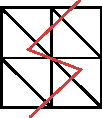
\includegraphics[height=2.2cm]{images/cutting-mig2015/remeshing_1.pdf}
\caption{\label{fig:remeshing1}}
\end{subfigure}
\hfill
\begin{subfigure}[c]{0.3\linewidth}
\centering
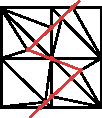
\includegraphics[height=2.2cm]{images/cutting-mig2015/remeshing_2.pdf}
\caption{\label{fig:remeshing2}}
\end{subfigure}
\hfill
\begin{subfigure}[c]{0.3\linewidth}
\centering
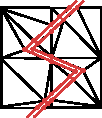
\includegraphics[height=2.2cm]{images/cutting-mig2015/remeshing_3.pdf}
\caption{\label{fig:remeshing3}}
\end{subfigure}
\caption{\label{fig:remeshing} Illustration of our remeshing algorithm. (a) For remeshing, we start from an input mesh and a polyline that represents the cut. (b) First we re-mesh along the polyline so that the mesh is conform with the cut. (c) Then we split the mesh vertices along the polyline.}
\end{figure}

\begin{figure}[p]
\centering
\begin{subfigure}[c]{0.3\linewidth}
\centering
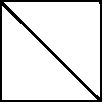
\includegraphics[height=2.2cm]{images/cutting-mig2015/basic_mesh.pdf}
\caption{\label{fig:basicMesh}}
\end{subfigure}
\hfill
\begin{subfigure}[c]{0.3\linewidth}
\centering
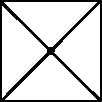
\includegraphics[height=2.2cm]{images/cutting-mig2015/edge_split.pdf}
\caption{\label{fig:edgeSplitting}}
\end{subfigure}
\hfill
\begin{subfigure}[c]{0.3\linewidth}
\centering
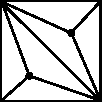
\includegraphics[height=2.2cm]{images/cutting-mig2015/vertex_insertion.pdf}
\caption{\label{fig:vertexInsertion}}
\end{subfigure}
\caption{\label{fig:operations} Illustrations for edge splitting and vertex insertions. (a) The input mesh. (b) After edge splitting. (c) After vertex insertions.}
\end{figure}

\begin{figure}[p]
\centering
\begin{subfigure}[c]{0.3\linewidth}
\centering
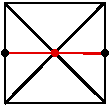
\includegraphics[height=2.2cm]{images/cutting-mig2015/vertex_splitting_1.pdf}
\caption{\label{fig:vertexSplitting1}}
\end{subfigure}
\begin{subfigure}[c]{0.3\linewidth}
\centering
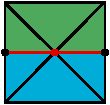
\includegraphics[height=2.2cm]{images/cutting-mig2015/vertex_splitting_2.pdf}
\caption{\label{fig:vertexSplitting2}}
\end{subfigure}
\begin{subfigure}[c]{0.3\linewidth}
\centering

\includegraphics[height=2.2cm]{images/cutting-mig2015/vertex_splitting_3.pdf}
\caption{\label{fig:vertexSplitting3}}
\end{subfigure}
\caption{\label{fig:vertexSplitting} Illustrations for the vertex splitting operation. (a) A mesh which is conform with the polyline (in red). (b) We start by assigning each triangle arround the vertex to split to one side of the polyline. (c) We duplicate the vertex and modify each of the triangles accordingly to its side.}
\end{figure}








%%%%%%%%%%%%%%%%%%%%%%%%%%%%%%%%%%%%%%%%%%%%%%%%%%%%










\chapter{Fluid sculpting}
Interactive fluid sculpting.

\chapter{Storyboarding physical animations}
Semantic for physics-based animation.

\chapter{Conclusion}
A conclusion

%\appendix

%\chapter{Nice details}
%Some details

\backmatter
%\nocite{*}

\printbibliography

\listoffigures

\listofalgorithms
 
\listoftables

\end{document}
